\documentclass[12pt]{article}

% Author's up-front packages
\usepackage[T1]{fontenc}
\usepackage[utf8]{inputenc}

% Packages on template
\usepackage{amsmath, mathtools}
\usepackage{amsfonts}
\usepackage{amssymb}
\usepackage{graphicx}
\usepackage{colortbl}
\usepackage{xr-hyper}
\usepackage{hyperref}
\usepackage{longtable}
\usepackage{xfrac}
\usepackage{tabularx}
\usepackage{float}
\usepackage{siunitx}
\usepackage{booktabs}
\usepackage{caption}
\usepackage{pdflscape}
\usepackage{afterpage}

% ---- Author's choice to remove them ----
%\usepackage[round]{natbib}
%\usepackage{refcheck}

% Author's packages
\usepackage{cite}
\usepackage{indentfirst}
\usepackage{cleveref}
\usepackage{float}
\usepackage{xcolor}
\definecolor{shadecolorIM}{RGB}{0,200,0}
\definecolor{shadecolorT}{RGB}{0,191,255}
\definecolor{shadecolorDD}{RGB}{186,85,211}
\definecolor{shadecolorR}{RGB}{255,0,0}

\hypersetup{
    %bookmarks=true,			% show bookmarks bar?
    colorlinks=true,			% false: boxed links; true: colored links
    linkcolor=red,				% color of internal links (change box color with 
%linkbordercolor)
    citecolor=green,        % color of links to bibliography
    filecolor=magenta,      % color of file links
    urlcolor=blue           % color of external links
}

%% Comments

\usepackage{color}

\newif\ifcomments\commentstrue

\ifcomments
\newcommand{\authornote}[3]{\textcolor{#1}{[#3 ---#2]}}
\newcommand{\todo}[1]{\textcolor{red}{[TODO: #1]}}
\else
\newcommand{\authornote}[3]{}
\newcommand{\todo}[1]{}
\fi

\newcommand{\wss}[1]{\authornote{blue}{SS}{#1}}
\newcommand{\an}[1]{\authornote{magenta}{Author}{#1}}


% For easy change of table widths
\newcommand{\colZwidth}{1.0\textwidth}
\newcommand{\colAwidth}{0.13\textwidth}
\newcommand{\colBwidth}{0.82\textwidth}
\newcommand{\colCwidth}{0.1\textwidth}
\newcommand{\colDwidth}{0.05\textwidth}
\newcommand{\colEwidth}{0.8\textwidth}
\newcommand{\colFwidth}{0.17\textwidth}
\newcommand{\colGwidth}{0.5\textwidth}
\newcommand{\colHwidth}{0.28\textwidth}


% Used so that cross-references have a meaningful prefix
\newcommand{\progname}{STEM Moir{\'e} GPA}

\usepackage{fullpage}

%Set the custom referencing system (author's initiative)
	% Goal Statement
\newtheorem{GS}{GS}
\crefname{GS}{GS}{GSs}
	% Assumption
\newtheorem{A}{A}
\crefname{A}{A}{As}
	% Theoretical Model
\newtheorem{T}{T}
\crefname{T}{T}{Ts}
	% Data Definition
\newtheorem{DD}{DD}
\crefname{DD}{DD}{DDs}
	% Data Constraints
\newtheorem{DC}{DC}
\crefname{DC}{DC}{DCs}
	% Instance Model
\newtheorem{IM}{IM}
\crefname{IM}{IM}{IMs}
	% General Definition
\newtheorem{GD}{GD}
\crefname{GD}{GD}{GDs}
	% Requirement
\newtheorem{R}{R}
\crefname{R}{R}{Rs}
	% Non Functional Requirement
\newtheorem{NR}{NR}
\crefname{NR}{NR}{NRs}
	% Likely change
\newtheorem{LC}{LC}
\crefname{LC}{LC}{LCs}

\begin{document}


\title{Software Requirements Specifications (SRS) \\
STEM Moir{\'e} GPA} 
\author{Alexandre Pofelski \\
		macid: pofelska \\
		github: slimpotatoes}
\date{\today}

\maketitle

\clearpage

\pagenumbering{roman}
\tableofcontents

\clearpage

\section{Revision History}

\begin{table}[h]
\caption{\bf Revision History}
\begin{tabularx}{\textwidth}{p{3cm}p{2cm}X}
\toprule {\bf Date} & {\bf Version} & {\bf Notes}\\
\midrule
4/10/2017 & 1.0 & First Draft\\
17/10/2017 & 1.1 & Significant corrections addressing comments and mistakes\\
18/10/2017 & 1.2 & Modification of \cref{IM_3} algorithm considered not enough precise\\
22/10/2017 & 1.2 & Few minor corrections\\
23/10/2017 & 1.3 & Fix a mistake in \cref{IM_4}\\
5/11/2017 & 1.3 & Some typos fixed\\
\bottomrule
\end{tabularx}
\end{table}

\clearpage

\section{Reference Material}

\subsection{Table of Units}

Throughout this document SI 
(\href{<https://physics.nist.gov/cuu/Units/index.html>}{Syst\`{e}me 
Internationale d'Unit\'{e}s}) is employed as the unit system. In addition to the 
basic units, several derived units are used as described below.  For each unit, 
the symbol is given followed by a description of the unit and the SI name.\par 
\bigskip

\renewcommand{\arraystretch}{1.2}
%\begin{table}[ht]
  \noindent \begin{tabular}{l l l} 
    \toprule		
    \textbf{Symbol} & \textbf{Base quantity} & \textbf{Name SI}\\
    \midrule 
    \si{\metre} & length & metre\\
    \si{\per\metre} & reciprocal meter & wave number\\
    \bottomrule
  \end{tabular}
  %	\caption{Provide a caption}
%\end{table}

\subsection{Table of Symbols}

The table that follows summarizes the symbols used in this document along with
their units if applicable.

%\renewcommand{\arraystretch}{1.2}
\noindent 
\begin{longtable*}{l l p{12cm}} 
\toprule
\textbf{Symbol} & \textbf{Unit} & \textbf{Description}\\
\midrule
\endhead
$\mathcal{B}$ & & 2D orthonormal base \\
$\mathcal{C}$ & & Ceiling function \\
$\delta$ & & Dirac delta function \\
$\Delta \overrightarrow{g_{j}}^{M_{\text{exp}}}$ & \si{\per\nano\meter} & Variation of
the $j^{\text{th}}$ Moir{\'e} wave vector of $\mathit{SMH}_{\text{exp}}$ \\
$\Delta \overrightarrow{g_{j}}^{C_{\text{exp}}}$ & \si{\per\nano\meter} & Variation of the $j^{\text{th}}$ crystalline wave vector of $\mathit{SMH}_{\text{exp}}$\\
$\varepsilon$ & & Strain tensor \\
$\varepsilon_{\mathit{xx}}$ & & Uniaxial strain component along $\vec{u_x}$ \\
$\varepsilon_{\mathit{yy}}$ & & Uniaxial strain component along $\vec{u_y}$ \\
$\varepsilon_{\mathit{xy}}$ & & Shear strain component in base $\mathcal{B}$ \\
$\mathcal{FT}$ & & Fourier transform \\
$\Gamma$ & & Spatial frequency range \\
$\overrightarrow{g_{j}}$ & \si{\per\nano\meter} & $j^{\text{th}}$ wave vector \\
$g_{j_x}$ & \si{\per\nano\meter} & Component of the $j^{\text{th}}$ wave vector along $\vec{u_x}$ \\
$g_{j_y}$ & \si{\per\nano\meter} & Component of the $j^{\text{th}}$ wave vector along $\vec{u_y}$ \\
$\overrightarrow{g_{j}}^{C}$ & \si{\per\nano\meter} & $j^{th}$ crystalline wave vector \\
$\overrightarrow{g_{j}}^{C_{\text{ref}}}$ & \si{\per\nano\meter} & $j^{\text{th}}$ crystalline wave vector of $I_{C_{\text{ref}}}$ \\
$\overrightarrow{g_{j}}^{C_{\text{exp}}}$ & \si{\per\nano\meter} & $j^{\text{th}}$ crystalline wave vector of $\mathit{SMH}_{\text{exp}}$\\
$\overrightarrow{g_{j}}^{C_{\text{exp}}}_{\text{uns}}$ & \si{\per\nano\meter} & $j^{\text{th}}$ crystalline wave vector of $\mathit{SMH}_{\text{exp}}$ at its unstrained state\\
$\overrightarrow{g_{j}}^{M_{\text{exp}}}$ & \si{\per\nano\meter} & $j^{\text{th}}$ Moir{\'e} wave vector of $\mathit{SMH}_{\text{exp}}$\\
$\overrightarrow{g_{j}}^{M_{\text{exp}}}_{\text{uns}}$ & \si{\per\nano\meter} & $j^{\text{th}}$ Moir{\'e} wave vector of $\mathit{SMH}_{\text{exp}}$ at its unstrained state\\
$i$ & & Imaginary unit \\
$I$ & & Intensity (or number of counts) \\
$\mathbb{I}$ & & Sub-set of $\mathbb{R}$ representing the position of the pixels in an image\\
$I_{C_{\text{ref}}}$ & & 2D array representing the reference crystal structure \\
$I_{\mathit{SMH}_{\text{exp}}}$ & & 2D array representing the experimental SMH\\
$I_{\mathit{SMH}_{\text{sim}}}$ & & 2D array representing the simulated SMH\\
$I_{\varepsilon_{\mathit{xx}}}$ & & 2D array representing the uniaxial strain component along $\vec{u_x}$ \\
$I_{\varepsilon_{\mathit{yy}}}$ & & 2D array representing the uniaxial strain component along $\vec{u_y}$ \\
$I_{\varepsilon_{\mathit{xy}}}$ & & 2D array representing the shear strain component in base $\mathcal{B}$ \\
$I_{\omega_{\mathit{xy}}}$ & & 2D array representing the rotation component in base $\mathcal{B}$ \\
$M_j$ & & Mask function in Fourier space including the $j^{\text{th}}$ wave vector\\
$\mathbb{N}$ & & Set of natural numbers\\
$\nabla$ & & Gradient operator\\
$\nabla u$ & & Displacement gradient tensor\\
$\vec{\nu}$ & \si{\per\nano\meter} & Vector position in Fourier space\\
$\omega$ & & Rotation tensor\\
$O$ & & Origin of the coordinate system \\
$\omega_{\text{xy}}$ & rad & Rotation element of the rotation tensor\\
$p$ & \si{\nano\meter} & Pixel size\\
$P_{\overrightarrow{X}}$ & rad & 2D array representing $2\pi\overrightarrow{X}\cdot\vec{r}$\\
$\overrightarrow{q_{n_j,m_j}}$ & & Sampling vector $\vec{q} \in Q$ of couple $(n_j,m_j)$\\
$Q$ & & Set such that $Q=\{\forall (n,m) \in \mathbb{Z}^{2}, \vec{q}=n\vec{u_x}+m\vec{u_y}\}$ \\
$\vec{r}$ & \si{\nano\meter} & Vector position \\
$\mathbb{R}$ & & Set of real numbers \\
$\overrightarrow{\mathit{rot}}$ & & Curl operator\\
$\mathit{SMH}_{\text{exp}}$ & & 2D array representing the experimental STEM Moir{\'e} Hologram \\
$\mathit{SMH}_{\text{sim}}$ & & 2D array representing the simulated STEM Moir{\'e} Hologram \\
$\vec{u_x}$ & & Unitary vector from base $\mathcal{B}$ \\
$\vec{u_y}$ & & Unitary vector from base $\mathcal{B}$ \\
$\wedge$ & & Mathematical symbol for "and"\\
$\bigwedge$ & & Cross product operator\\
$\mathbb{Z}$ & & Set of integer numbers\\
\bottomrule
\label{table_symbols_SRS}
\end{longtable*}

\subsection{Abbreviations and Acronyms}

\renewcommand{\arraystretch}{1.2}
\begin{tabular}{l l} 
  \toprule		
  \textbf{symbol} & \textbf{description}\\
  \midrule 
  A & Assumption\\
  AU & Arbitrary Unit\\
  DC & Data Constraint \\
  DD & Data Definition\\
  EM & Electron Micrograph \\
  GD & General Definition\\
  GPA & Geometrical Phase Analysis \\
  GS & Goal Statement\\
  IM & Instance Model\\
  LC & Likely Change\\
  PS & Physical System Description\\
  NR & Non functional Requirement\\
  R & Requirement\\
  SMH & STEM Moir{\'e} Hologram \\
  SRS & Software Requirements Specification\\
  STEM & Scanning Transmission Electron Microscopy \\
  T & Theoretical Model\\
  \bottomrule
  \label{table_acro_SRS}
\end{tabular}

\newpage
\pagenumbering{arabic}

\section{Introduction}

\subsection{Purpose of Document}

The purpose of the document is to provide a detailed description of the functional and the non-functional requirements of the \progname{} software.  The theoretical models on which the requirements are based on are also described to provide the context of each instance model.

\wss{The text is better for version control, and for reading in other editors,
  if you use a hard-wrap at 80 characters}
\an{I understand the point. My tex editor is not so friendly with the 80 characters hard wrap (especially with equations) so I avoided it. I will try to find a solution}

\subsection{Scope of Requirements} 

The scope of requirements are limited to the realization of \cref{GS_1} which corresponds to transform a certain type of data to another one based on multiple user inputs. \progname{} is for the moment limited to the study of mono-crystalline material undergoing a relative small deformation with respect to its unstrained state.

\subsection{Characteristics of Intended Reader} 

The intended reader is expected to have a minimum knowledge in mathematics at
undergraduate level. Simplification of some physical concepts are proposed to
make the document technically accessible. Nevertheless, a basic knowledge in
Transmission Electron Microscopy, electron/matter interaction and elastic strain
theory is recommended to get a deeper understanding of the document. \wss{Is
  there are standard textbook, or other resource, you can point to?}

\subsection{Organization of Document}

The document follows the template of the SRS document proposed by \cite{SmithAndLai2005, SmithEtAl2007}. 

\section{General System Description}

This section identifies the interfaces between the system and its environment,
describes the user characteristics and lists the system constraints.

\subsection{System Context}

\progname{} is intended to transform specific data acquired from the microscope into physical information related to the sample analysed. The variety of samples is potentially huge therefore to cover the maximum of cases, multiple interactions with the user are required to process the data correctly. Responsibilities between the user and the \progname{} are described as follows:

\begin{itemize}
\item User Responsibilities:
\begin{itemize}
\item Provide the minimum information required by the \progname{} software.
\item Use the software in the limits it is intended to by respecting \cref{A_4}, \cref{A_5}, \cref{A_6} and \cref{A_7}.
\item Be aware of the potential effects of user inputs on the quality of the final data.
\item Judge the correctness of the data.
\item Be particularly cautious on the use of the final data quantitatively. The quantitative aspect cannot be fully uncorrelated from the user inputs. 
\item Use a pointing device, a keyboard and a display to interface with \progname{}.
\end{itemize}
\item \progname{} Responsibilities:
\begin{itemize}
\item Inform the user of their responsibilities in using \progname{}.
\item Preserve the integrity of original data and not add any hidden processing steps on the final data such as, but not limited to, smoothing, blurring, averaging, de-noising and binning.
\item Inform user of wrong format or missing information regarding the inputs.
\item Inform the user of a potential insufficient quality of the final results which could lead to non reliable physical interpretations.
\end{itemize}
\end{itemize}

\wss{We will touch on it later when we discuss Assurance Cases, but you might
  add a responsibility to the system to explicitly warn the user of their
  responsibilities.  This is analogous to an electrical device that has a
  warning to read the manual before operating.}
\an{I like the idea. I will add it in the responsibilities but will let the comment for further discussion}

\subsection{User Characteristics} \label{SecUserCharacteristics}

The end user of \progname{} should have a relative strong background in Physics (interaction electron/matter) and Mathematics (or signal processing) at graduate level to get a reliable sense of the data processed. The multiple interactions between the user and \progname{} have  significant impact on the final results which can lead to some physical misinterpretations. Basic practical and theoretical knowledge in Electron Microscopy is recommended because of the terminology used in the document. 

\subsection{System Constraints}

To be considered by the electron microscopy community, \progname{} has to be able to read dm3 files format, an non-standard format used by the electron detector manufacturer. 

\section{Specific System Description}
\subsection{Problem Description} \label{Sec_pd}

STEM Moir{\'e} GPA project is a software capable of converting a STEM Moir{\'e} hologram into 2D relative strain maps. Terminologies and the physical system are described below.

\subsubsection{Terminology and Definitions}

Regarding the complexity of the electron/matter interaction, some crude  simplifications are proposed to describe the terminologies below. While sometimes not realistic, the simplifications should help in visualizing the context and the type of data the STEM Moir{\'e} GPA software is subjected to. Nevertheless, all the simplifications proposed are not affecting the definition of the concept used at the software level.

\begin{itemize}

\item \textbf{2D Cartesian coordinate system}: orthonormal coordinate system model by the base $\mathcal{B}=(O,\vec{u_x},\vec{u_y})$ with $O$ representing the origin and $M$ a point with coordinate the $(x,y)$, such that any vector $\vec{r}=\overrightarrow{\mathit{OM}}$ can be expressed as the following :
\begin{equation}
\forall (x,y) \in \mathbb{R}^{2}, \vec{r}=x\vec{u_x}+y\vec{u_y}
\end{equation}
\item \textbf{Pixel}: smallest addressable element sampling a 2D continuum.
\item \textbf{Detector}: Element in \cref{fig:STEM_imaging_Fig} collecting and counting the electron that crossed the sample.
\item \textbf{Electron Micrograph (EM)}: 2D array collected in an electron microscope representing the number of electron crossing the sample (intensity) at each pixel location.
\item \textbf{Scanning grid}: set representing the succession of the STEM probe positions when collecting the STEM EM. Equivalently the scanning grid represents the relative position of the pixel with respect to the sample when acquiring the EM. A simplified version of the 
STEM EM formation can be visualized in \cref{fig:STEM_imaging_Fig}. The positions of the STEM probe are located at the intersection of the black grid lines.
\begin{figure}[H]
\begin{center}
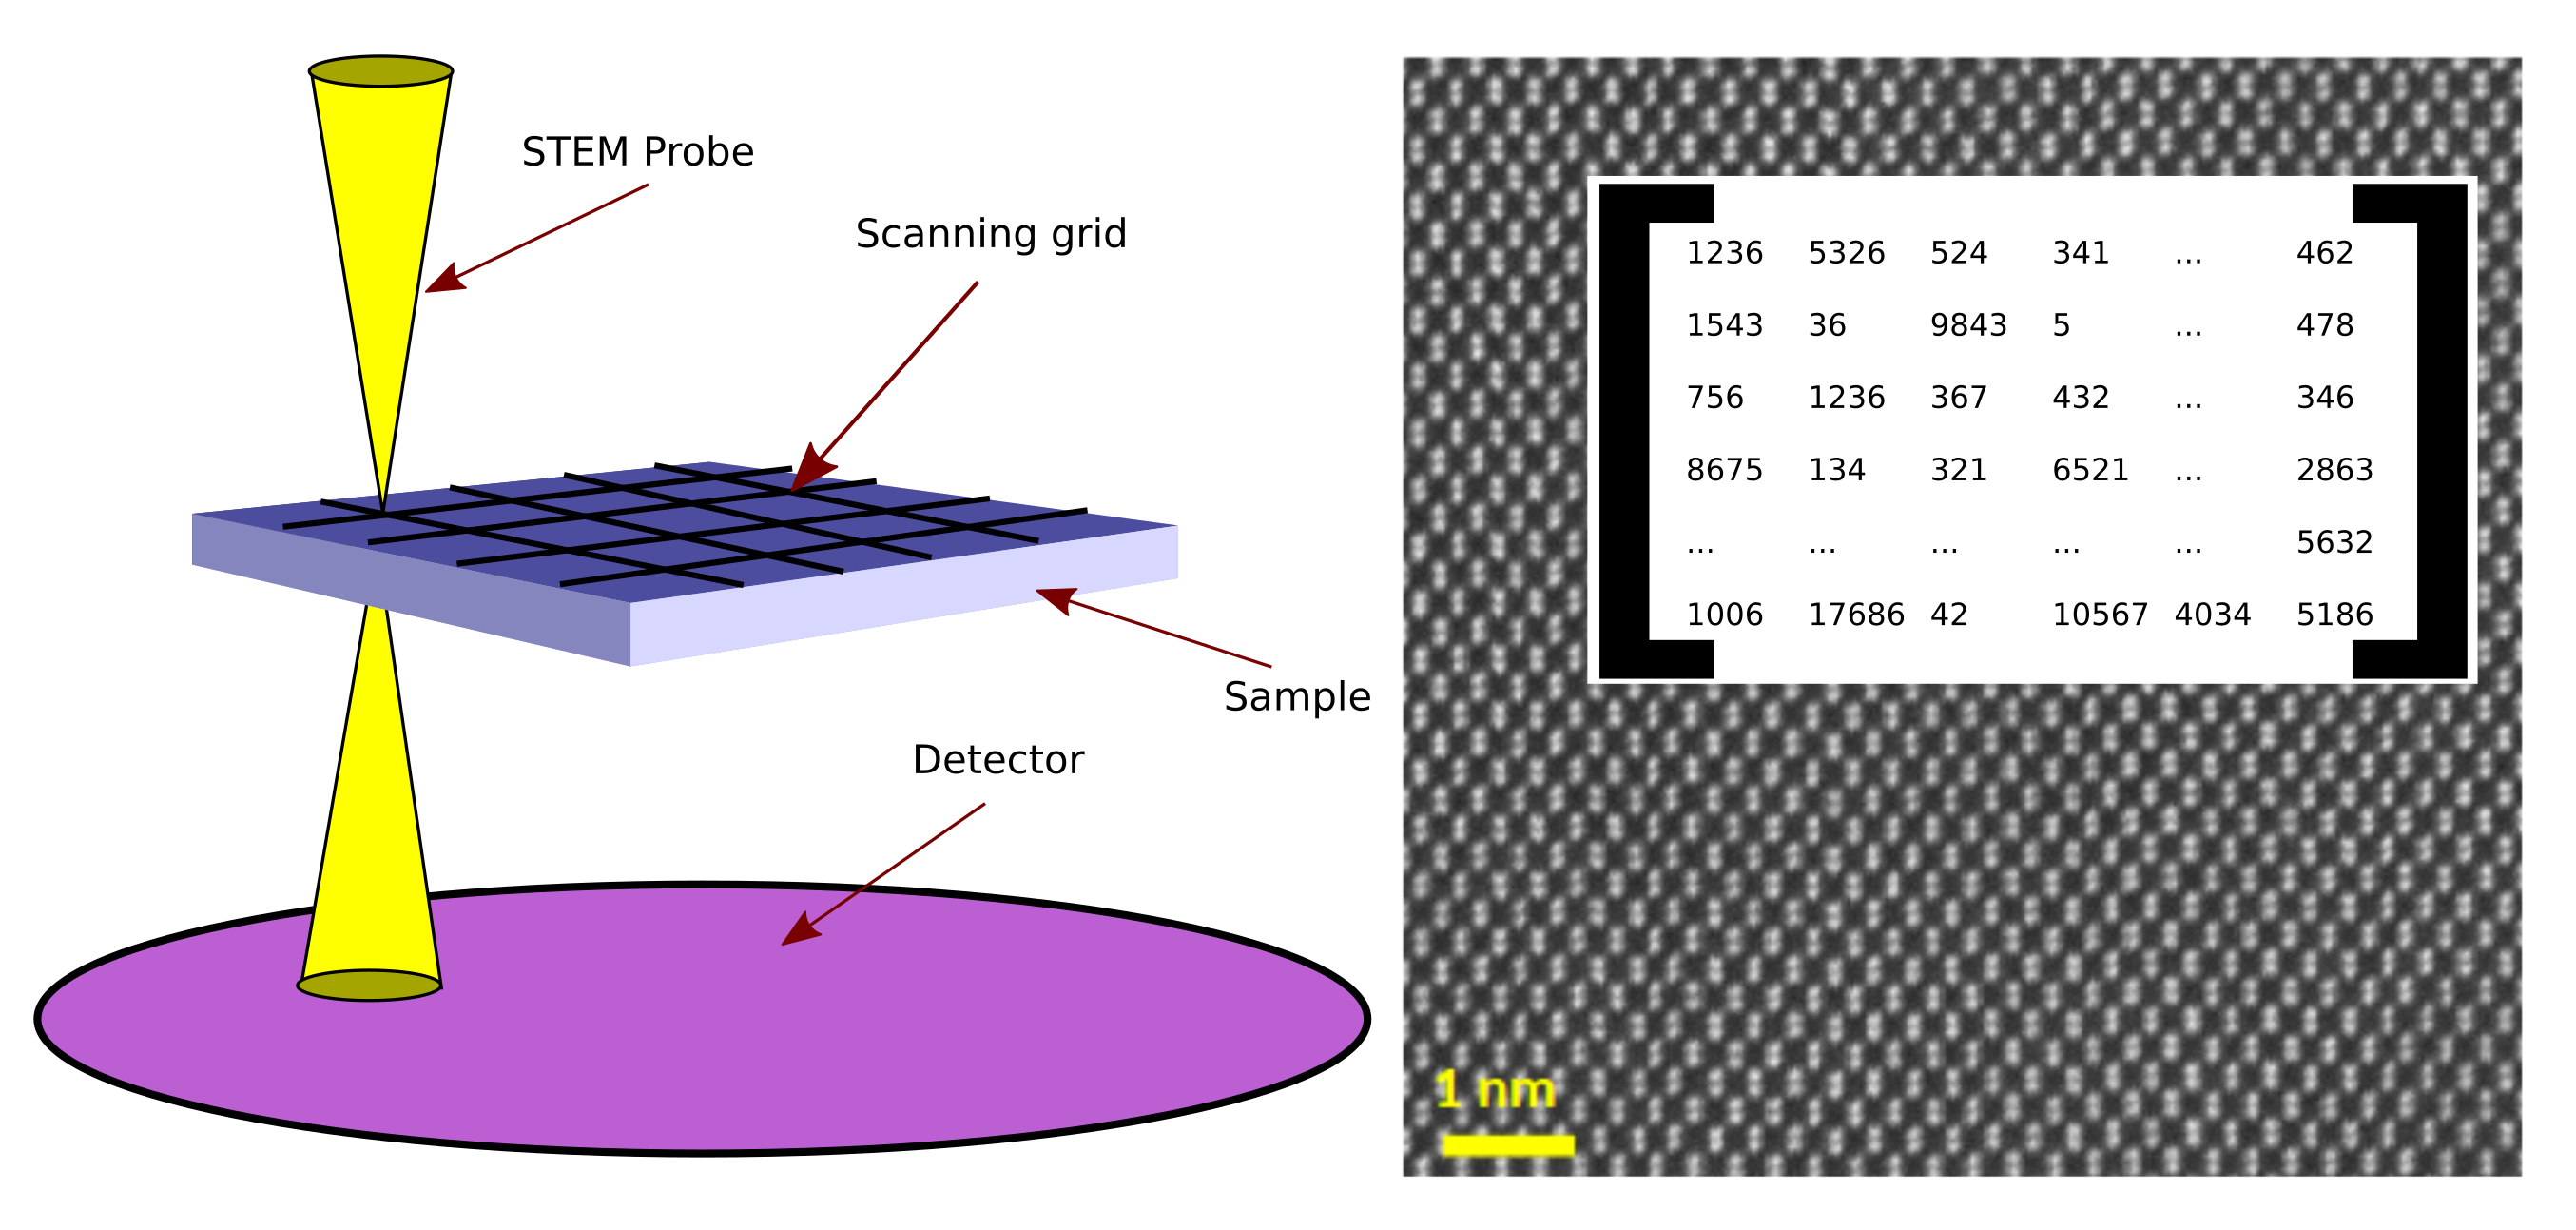
\includegraphics[scale=0.7]{Figures/STEM_imaging_Fig.png}
\caption{(Left) Schematic of the STEM EM formation with the STEM probe scanning the sample at each intersection of the grid lines. The electrons crossing the sample are collected on the detector and counted during the acquisition time. (Right) STEM EM on a pure silicon sample revealing its atomic structure. In the inset is highlighted the type of data the STEM EM corresponds to which is a 2D array with the intensity collected on each pixel.}
\label{fig:STEM_imaging_Fig}
\end{center}
\end{figure}
\item \textbf{Hologram}: Result from an interference between two or multiples waves. \newline
Let consider two monochromatic plane waves $\psi_1$ and $\psi_2$ with their respective amplitude $A_j$, phase $\phi_j$ and wave vector $\vec{k_j}$ in the 2D Cartesian system interfering with each other. The resulting hologram $\psi_H$  can be modelled as follows with :
\begin{equation}
\forall (x,y) \in \mathbb{R}^{2}, \psi_H(\vec{r})=\psi_1+\psi_2= A_1e^{i(\vec{k_1}\cdot\vec{r})+i\phi_1}+A_2e^{i(\vec{k_2}\cdot\vec{r})+i\phi_2}
\end{equation}
The intensity $I_H$ can be calculated as follows, with $\psi_H^{*}$ representing the complex conjugate of $\psi_H$
\begin{equation}
\begin{split}
\forall (x,y) \in \mathbb{R}^{2}, I_H(\vec{r})=\psi_H\psi_H^{*}= & A_{1}^{2}+A_{2}^{2}+ \\ & A_{1}A_{2}(e^{i(\vec{k_1}-\vec{k_2})\cdot\vec{r}+i(\phi_1-\phi_2)}+e^{i(\vec{k_2}-\vec{k_1})\cdot\vec{r}+i(\phi_2-\phi_1)})
\end{split}
\label{eq:hologram}
\end{equation}
The more waves are contributing to the hologram, the more complex \cref{eq:hologram} will be. However, similar factors will appear with constants and cross product terms.
\item \textbf{Moir{\'e} hologram}: Result from interference between two or multiple waves with similar but not equal wave numbers (or wave vectors in 2D).
\item \textbf{Crystal lattice}: Periodic arrangement of atoms forming matter.
\item \textbf{STEM Moir{\'e} hologram (SMH)}: EM collected in STEM and resulting from the 
Moir{\'e} interference between the scanning grid and the crystal lattice. 
\item \textbf{Strain map}: 2D array mapping the evolution of one element of the 2D strain or rotation 
tensor. 
\end{itemize}

\subsubsection{Physical System Description}

The physical system of \progname{}, as shown in \cref{fig:system_description}, includes the following elements:
\begin{itemize}
\item The STEM Moir{\'e} hologram as the results of the interaction between the scanning grid and the crystal periodicity of the sample.
\item Physical inputs provided by the user to convert a STEM Moir{\'e} hologram into strain and rotation maps.
\end{itemize}

\begin{figure}[H]
\begin{center}
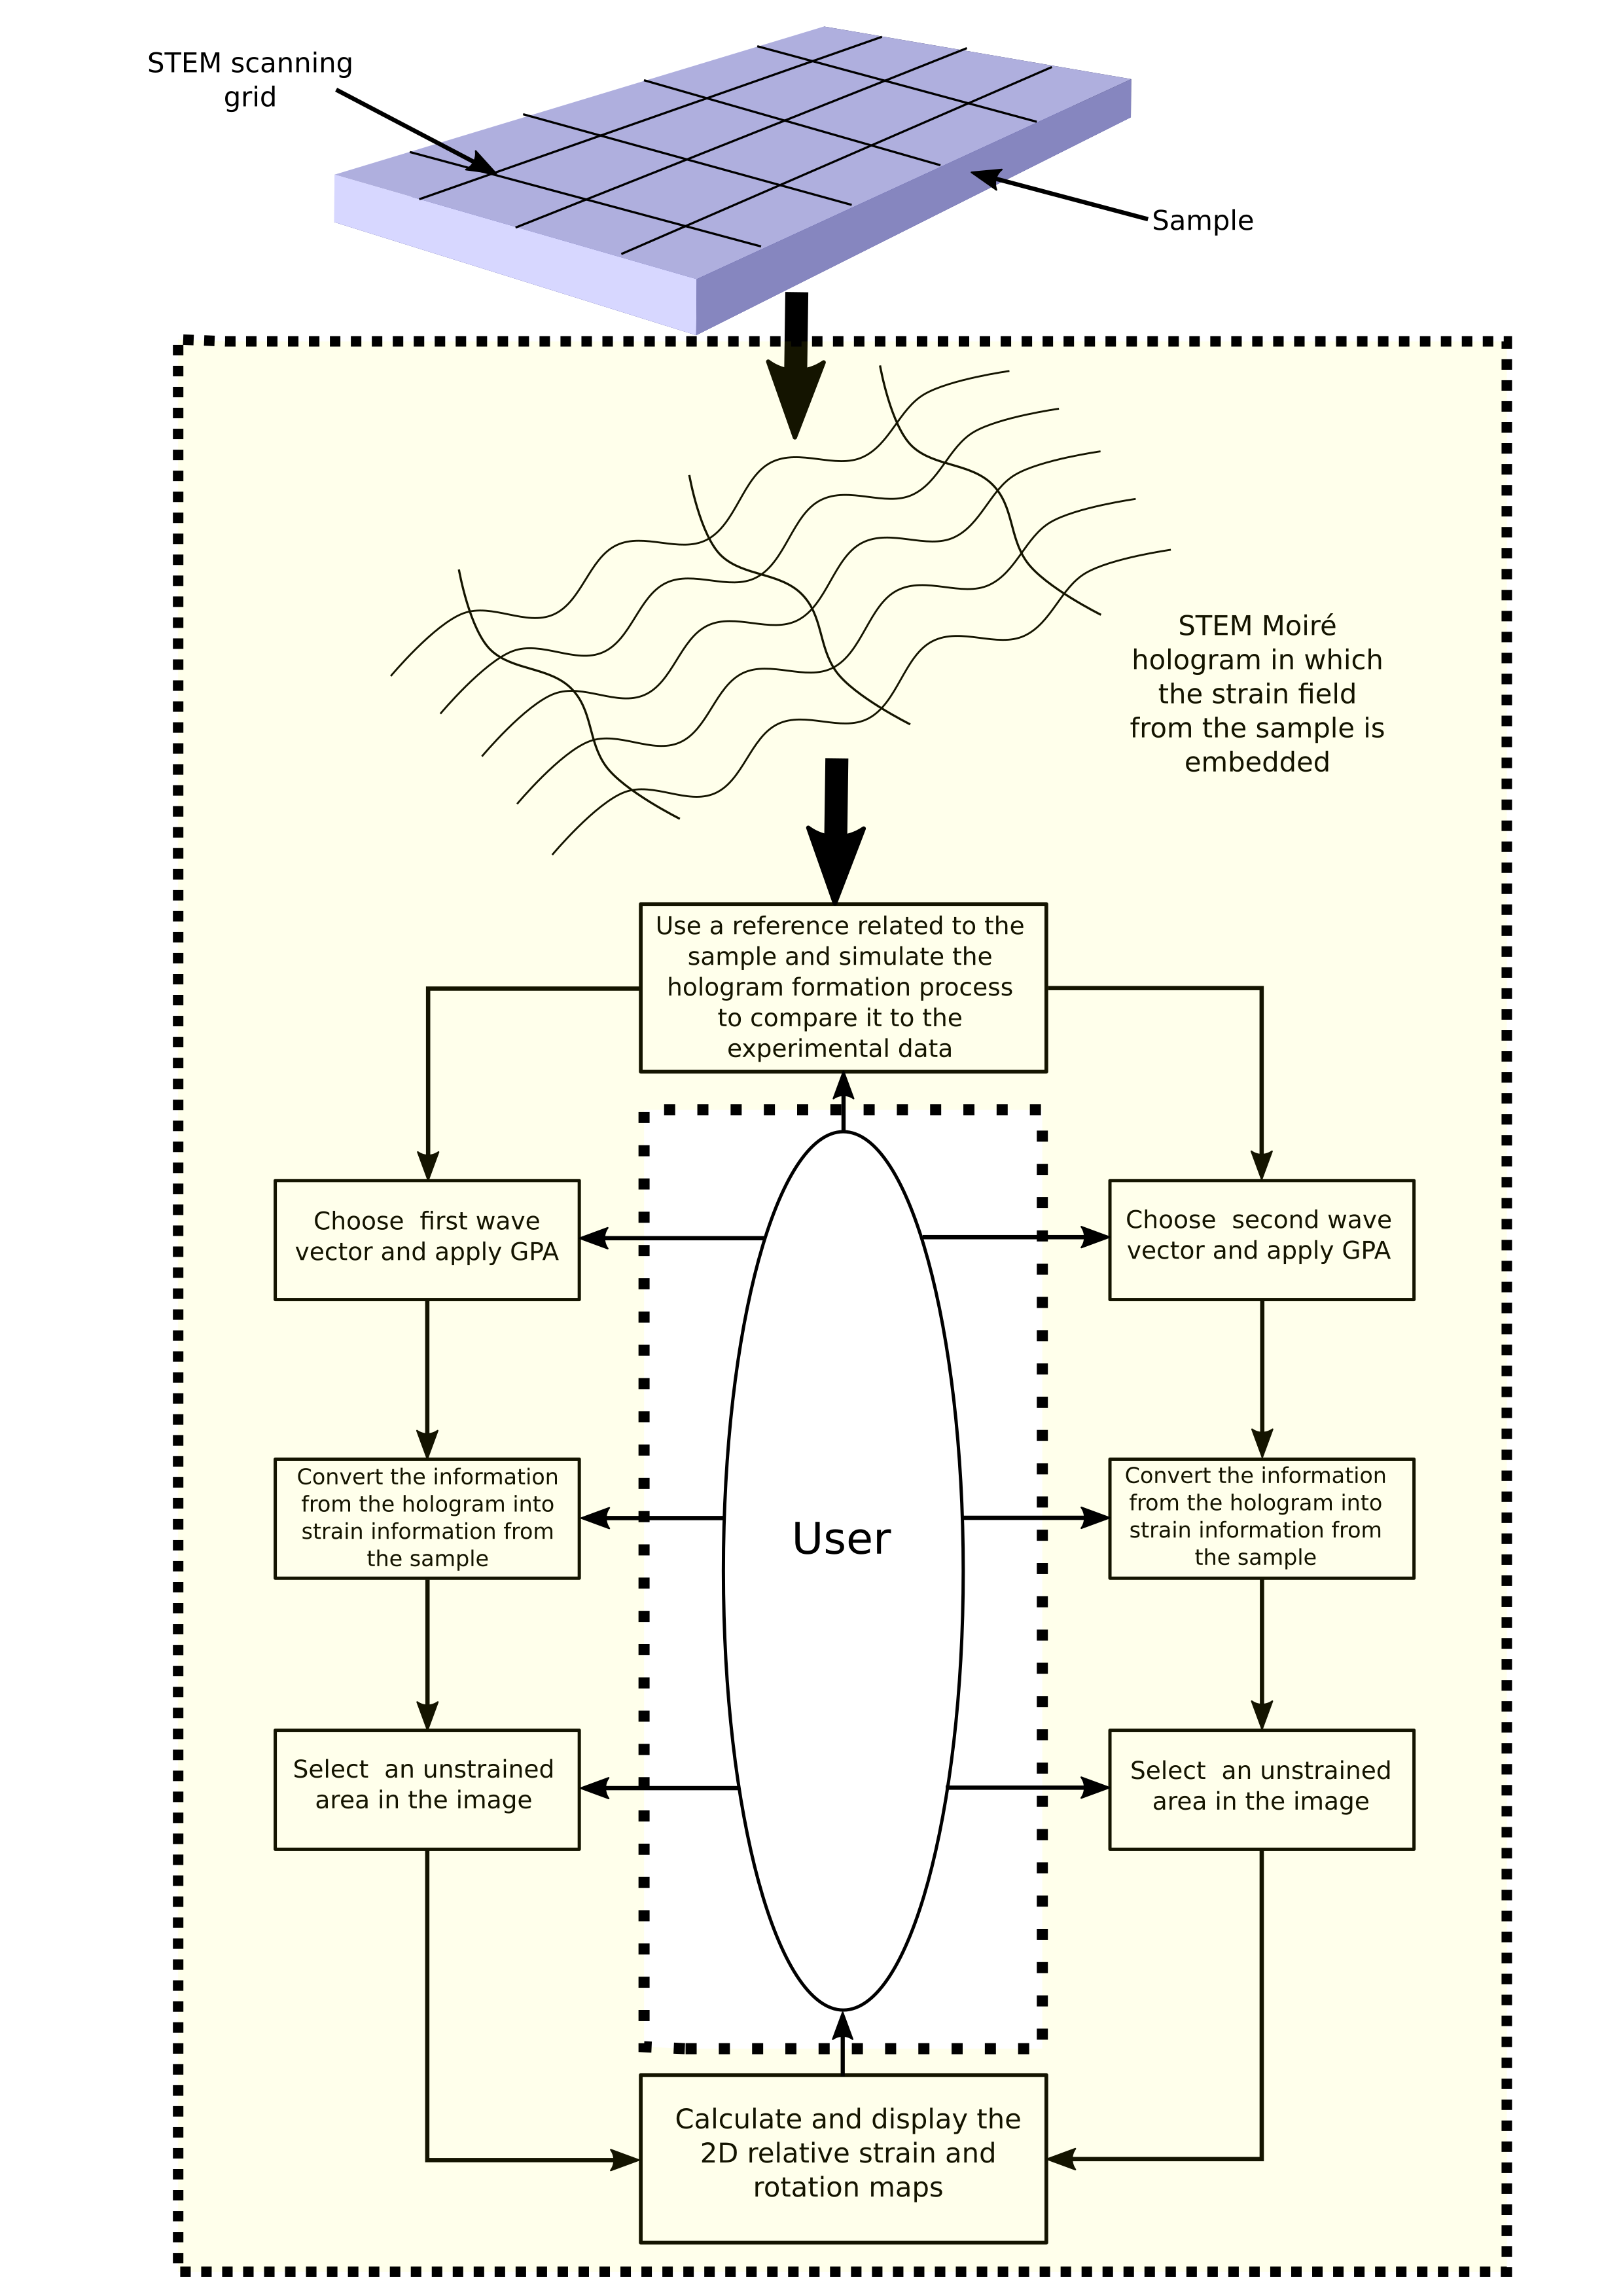
\includegraphics[scale=0.65]{Figures/System_description.png}
\caption{Physical system of \progname{} highlighted in the yellow area.}
\label{fig:system_description}
\end{center}
\end{figure}

\subsubsection{Goal Statements}
\noindent Given the system description, the goal statement is:
\begin{GS}
\normalfont Extract and display the relative 2D strain field from a STEM Moir{\'e} hologram.
\label{GS_1}
\end{GS}

\subsection{Solution Characteristics Specification}

\subsubsection{Assumptions}

\begin{A}
\normalfont The microscope has a limit in resolution corresponding to the probe size and thus cannot resolve any spatial frequency higher than $g_{j_{\text{lim}}}$. 
\label{A_1}
\end{A}
\begin{A}
\normalfont Since the STEM EM is discretized in pixels, the smallest feature detectable is composed of two pixels. Therefore, in reciprocal space, the maximum range of spatial frequency detectable is $\Gamma=[-\frac{1}{2p},\frac{1}{2p}]^{2}$.
\label{A_2}
\end{A}
\begin{A}
\normalfont The probe size is smaller than the area covered by one pixel. Therefore, information gathered on one pixel is only provided by the area covered by the pixel (no blurring) and \cref{A_1} is the only limiting factor regarding resolution.
\label{A_3}
\end{A}
\begin{A}
\label{A_4}
\normalfont The gradient of the deformation field is small. Therefore,
\begin{equation*}
\begin{gathered}
\forall \vec{r} \in \mathbb{R}^2, \ \nabla (\Delta\overrightarrow{g_j}\cdot\vec{r})= (\Delta\overrightarrow{g_j}\cdot\nabla)\vec{r}+(\vec{r}\cdot\nabla)\Delta\overrightarrow{g_j}+\Delta\overrightarrow{g_j}\bigwedge \overrightarrow{\mathit{rot}}(\vec{r})+\vec{r}\bigwedge \overrightarrow{\mathit{rot}}(\Delta\overrightarrow{g_j}))\\
\forall \vec{r} \in \mathbb{R}^2, \ \nabla (\Delta\overrightarrow{g_j}\cdot\vec{r})\approx \Delta\overrightarrow{g_j}
\end{gathered}
\end{equation*}
\end{A}
\begin{A}
\label{A_5}
\normalfont The deformation magnitude is small. Therefore, $\frac{||\Delta\overrightarrow{g_j} ||}{||\overrightarrow{g_j} ||}\leq 0.1$
\end{A}
\begin{A}
\label{A_6}
\normalfont The user knows the crystal structure of the sample analysed at its unstrained state or can provide a reference in which is embedded the crystal structure information at its unstrained state.
\end{A}
\begin{A}
\label{A_7}
\normalfont The sample, from which the SMH is acquired, is mono-crystalline.
\end{A}

\subsubsection{Theoretical Models}\label{sec_theoretical}

\begin{T}
\label{T_1}
\noindent\colorbox{shadecolorT}{\normalfont \textbf{2D periodic sampling}}
\normalfont
\begin{itemize}
\item \underline{Equation}: \Cref{eq:sampling_simplified}
\item \underline{Description}: In the 2D Cartesian coordinate system $\mathcal{B}$, the scanning grid can be seen as sampler $S$ sampling a continuous function $f$. In the context of the \progname{} project, the sampler is set to be periodic with the same periodicity $p$ (called pixel size) in both $x$ and $y$ directions (2D Dirac comb). The resulting sampled version $f_S$ of $f$ can be represented as the following with $\delta$ representing the Dirac function:
\begin{equation}
\begin{gathered}
\forall (x,y) \in \mathbb{R}^{2}, f_S(x,y)=S(x,y)\times f(x,y) \\
\forall (x,y) \in \mathbb{R}^{2}, f_S(x,y)=\sum_{n=-\infty}^{n=+\infty}\sum_{m=-\infty}^{m=+\infty}\delta(x-np,y-mp)\times f(x,y)
\end{gathered}
\label{eq:sampling}
\end{equation}
For shorter notations, it is possible to define a set Q as follows $Q=\{\forall (n,m) \in \mathbb{Z}^{2}, \vec{q}=n\vec{u_x}+m\vec{u_y}\}$ and thus simplify \cref{eq:sampling}
\begin{equation}
\forall (x,y) \in \mathbb{R}^{2}, f_S(\vec{r})=\sum_{q\in Q}\delta(\vec{r}-p\vec{q}) f(\vec{r})
\label{eq:sampling_simplified}
\end{equation}
\item \underline{Source}: \cite{Gonzalez_1992}
\item \underline{Ref by}: \cref{DD_2}, \cref{IM_1}, \cref{IM_4}
\end{itemize}
\end{T}

\begin{T}
\label{T_2}
\noindent\colorbox{shadecolorT}{\normalfont \textbf{Geometrical Phase Analysis}}
\normalfont
\begin{itemize}
\item \underline{Equation}: \Cref{eq:GPA_method}
\item \underline{Description}: Let consider a function $f$ decomposed in Fourier series as the following with 
\begin{equation}
\begin{gathered}
\forall \vec{r}=(x_1,...,x_n) \in \mathbb{R}^n, f(\vec{r})=\sum_{j=-\infty}^{j=+\infty}C_je^{i(\vec{k_j}\cdot\vec{r})} \\
\forall \vec{r}=(x_1,...,x_n) \in \mathbb{R}^n, f(\vec{r})=\sum_{j=-\infty}^{j=+\infty}A_je^{i((\vec{k_j}\cdot\vec{r})+B_j)}
\end{gathered}
\end{equation}
If there is a small perturbation locally of the n-dimensions wave vector $\vec{k_j}$, it is possible to model it by allowing $B_j$ to be a function of $\vec{r}$. 
\begin{equation}
\forall \vec{r}=(x_1,...,x_n) \in \mathbb{R}^n, f(\vec{r})=\sum_{j=-\infty}^{j=+\infty}A_je^{i((\vec{k_j}\cdot\vec{r})+B_j(\vec{r}))}
\end{equation}
The objective of GPA is to extract the perturbation (one chosen $B_j(\vec{r})$) from $f$ in Fourier space. Let's consider $\widetilde{f}$ the Fourier transform of $f$ such that
\begin{equation*}
\begin{gathered}
\forall \vec{\nu}=(\nu_1,...,\nu_n) \in \mathbb{R}^n, \forall \vec{r}=(x_1,...,x_n) \in \mathbb{R}^n, \widetilde{f}(\vec{\nu})=\mathcal{FT}(f(\vec{r})) \\
\forall \vec{\nu}=(\nu_1,...,\nu_n) \in \mathbb{R}^n, \forall \vec{r}=(x_1,...,x_n) \in \mathbb{R}^n, \widetilde{f}(\vec{\nu})=\sum_{j=-\infty}^{j=+\infty}\mathcal{FT}(C_j(\vec{r})\times e^{i(\vec{k_j}\cdot\vec{r})})
\end{gathered}
\end{equation*}
\begin{equation}
\begin{gathered}
\forall \vec{\nu}\in \mathbb{R}^n, \widetilde{f}(\vec{\nu})=\sum_{j=-\infty}^{j=+\infty}\widetilde{C_j}(\vec{\nu})\ast\delta(\vec{\nu}-\vec{k_j})\\
\forall \vec{\nu}\in \mathbb{R}^n, \widetilde{f}(\vec{\nu})=\sum_{j=-\infty}^{j=+\infty}\widetilde{C_j}(\vec{\nu}-\vec{k_j})
\end{gathered}
\end{equation}
If all the $\vec{k_j}$ are separated enough to be isolated with a mask, then $B_j(\vec{r})$ can be extracted by considering the inverse Fourier transform of the masked area and expressing the result in term of amplitude and phase. In mathematical formalism, $B_j(\vec{r})$ is extracted as follows with $\mathcal{G}=([\nu_1^D,\nu_1^U],...,[\nu_n^D,\nu_n^U])$ and $\nu_i^D, \nu_i^U$ two real numbers defining respectively the lower and the upper side of the interval $[\nu_i^D, \nu_i^U$].
\begin{equation*}
\begin{gathered}
\text{if} \ \exists \ M :
\begin{array}{|ccl}
\mathbb{R}^{n} & \longrightarrow & \mathbb{C} \\
\vec{\nu} & \longmapsto & M(\vec{\nu}) 
    \end{array} / \begin{cases}
    					M(\vec{\nu}-\vec{k_j})\widetilde{f}(\vec{\nu})=\widetilde{C_j}(\vec{\nu}-\vec{k_j}) & \text{for} \ \vec{\nu} \in \mathcal{G} \\
    					M(\vec{\nu}-\vec{k_j})\widetilde{f}(\vec{\nu})=0 & \text{for} \ \vec{\nu} \notin \mathcal{G}
    				 \end{cases} \\
\end{gathered}
\end{equation*}
\begin{equation}
\Rightarrow \begin{array}{l}
|\mathcal{FT}^{-1}[M(\vec{\nu})\widetilde{f}(\vec{\nu}+\vec{k_j})]|=|\mathcal{FT}^{-1}[\widetilde{C}(\vec{\nu})]|=A_j \\
\label{eq:GPA_method}
arg(\mathcal{FT}^{-1}[M(\vec{\nu})\widetilde{f}(\vec{\nu}+\vec{k_j})])=arg(\mathcal{FT}^{-1}[\widetilde{C}(\vec{\nu})])=B_j(\vec{r})
\end{array}
\end{equation}

\item \underline{Source}: \cite{Hytch1998,Rouviere2005}
\item \underline{Ref by}: \cref{DD_1}, \cref{IM_2}
\end{itemize}
\end{T}

\subsubsection*{Description of the GPA method in a 1D coordinate system}
\noindent Let's consider a function $f$ such that 
\begin{equation*}
\begin{gathered}
\forall x \in \mathbb{R}, f(x)=C_0e^{i(k_0x)}+C_1e^{i(k_1x)} \\
\end{gathered}
\end{equation*}
Let's consider a small perturbation of $k_1$ modelled as the following
\begin{equation*}
\begin{gathered}
\forall x \in \mathbb{R}, f(x)=C_0e^{i(k_0x)}+A_1e^{i(k_1x)+iB_1(x)} \\
\end{gathered}
\end{equation*}
Applying the GPA method on $f$,
\begin{equation*}
\begin{gathered}
\forall \nu \in \mathbb{R}, \widetilde{f}(\nu)=C_0\delta(\nu-k_0)+\widetilde{C_1}(\nu)\ast\delta(\nu-k_1) \\
\forall \nu \in \mathbb{R}, \widetilde{f}(\nu)=C_0\delta(\nu-k_0)+\widetilde{C_1}(\nu-k_1)
\end{gathered}
\end{equation*}
Considering the perturbation around $k_1$ to be small and that $k_0$ and $k_1$ are enough separated such that the perturbation is located around $k_1$ in frequency space, it is possible to define a mask $M$ and constant $\epsilon \in \mathbb{R}$ such that:
\begin{equation*}
\begin{gathered}
\forall \nu \in \mathbb{R}, M(\nu) = 
\begin{cases}
1 & \text{for} \ \nu-k_1 \in  [-\epsilon,+\epsilon] \ / \ k_0 \notin [k_1-\epsilon,k_1+\epsilon] \\
0
\end{cases}
\end{gathered}
\end{equation*}
In such case, multiply the mask $M$ with the Fourier transform of $f$ isolates $\widetilde{C_1}$ from the sum and can be independently transformed as follows:
\begin{equation*}
\begin{gathered}
\forall \nu \in \mathbb{R}, M(\nu-k_1)\widetilde{f}(\nu)=\widetilde{C_1}(\nu-k_1)
\end{gathered}
\end{equation*}
Setting, $\lambda=\nu-k_1$ and performing the inverse Fourier transform of the masked Fourier transform of $f$, the perturbation can be extracted.
\begin{equation*}
\begin{gathered}
\forall \nu \in \mathbb{R}, M(\lambda)\widetilde{f}(\lambda+k_1)=\widetilde{C_1}(\lambda) \\
\forall x \in \mathbb{R}, \mathcal{FT}^{-1}[M(\lambda)\widetilde{f}(\lambda+k_1)]=C_1(x) \\
\Rightarrow \begin{cases}
|C_1(x)|=A_1 \\
arg(C_1(x))=B_1(x)
\end{cases}
\end{gathered}
\end{equation*}
\begin{T}
\label{T_3}
\noindent\colorbox{shadecolorT}{\normalfont \textbf{Strain decomposition model}}
\normalfont
\begin{itemize}
\item \underline{Equation}: \Cref{eq:strain_2}
\item \underline{Description}: In infinitesimal strain theory with small displacement and small gradient of displacement (\cref{A_4}, \cref{A_5}), the displacement gradient tensor $\nabla u$ can be decomposed in two independent tensors: the symmetric strain tensor $\varepsilon$ and the anti-symmetric rotation tensor $\omega$. Their relationship can be described as follows:
\begin{equation}
\begin{gathered}
\nabla u = \varepsilon + \omega = \begin{bmatrix}
	\varepsilon_{\mathit{xx}} & \varepsilon_{\mathit{xy}} \\
	\varepsilon_{\mathit{xy}} & \varepsilon_{\mathit{yy}} 
	\end{bmatrix} + \begin{bmatrix}
	0 & \omega_{\mathit{xy}} \\
	-\omega_{\mathit{xy}} & 0 
	\end{bmatrix} \\ 
\varepsilon = \frac{1}{2}(\nabla u+(\nabla u)^{T}) \\
\omega = \frac{1}{2}(\nabla u-(\nabla u)^{T})
\end{gathered}
\label{eq:strain_2}
\end{equation}
\item \underline{Source}: \cite{Hytch1998,Rouviere2005}
\item \underline{Ref by}: \cref{DD_3}, \cref{IM_3}, \cref{IM_5}
\end{itemize}
\end{T}

\subsubsection{General Definitions}\label{sec_gendef}

No general definitions are needed for the current documentation.

\subsubsection{Data Definitions}\label{sec_datadef}

\renewcommand{\labelitemi}{$\star$}

\begin{DD}
\label{DD_1}
\noindent\colorbox{shadecolorDD}{\normalfont \textbf{Variation of the crystalline wave vector $\Delta \overrightarrow{g_j}$ (strain in crystal lattice)}}
\normalfont
\begin{itemize}
\item \underline{Equation}: \Cref{eq:Strain_GPA}
\item \underline{Description}: For the purpose of the STEM Moir{\'e} GPA, only mono-crystalline samples are analysed (\cref{A_7}). In the case of a perfect periodic atomic arrangement, the crystalline lattice $I_c$ can be described in Fourier series with $C_j$ the complex Fourier coefficient related to the crystalline wave vector $\vec{g_j}$ in the 2D Cartesian system $\mathcal{B}$.
\begin{equation}
\forall (x,y) \in \mathbb{R}^{2},I_C(\vec{r})=\sum_{j=-\infty}^{j=+\infty}C_je^{i(\vec{g_j}\cdot\vec{r})}
\label{eq:crystal_Fourier_series}
\end{equation}
If the crystal is deformed, the relative position of the atoms will be slightly modified from their original unstrained configuration. The local deformation is breaking locally the perfect periodicity of the crystalline lattice. In the case of small deformation (\cref{A_5}), $C_j$ can be allowed to vary in space in \cref{eq:crystal_Fourier_series}. Representing $C_j$ with a phase $A_j$ and an amplitude $P_j$, a pure displacement is only contributing in the phase component. The strain information is therefore embedded in $P_{g_{j}}(\vec{r})$ such that $P_{g_{j}}(\vec{r})=2\pi\Delta \overrightarrow{g_{j}}(\vec{r})\cdot\vec{r}$ where $\Delta \overrightarrow{g_j}$ represent the variation of the crystalline vector compared to its unstrained state.
\begin{equation}
\begin{gathered}
\forall (x,y) \in \mathbb{R}^{2},I_C(\vec{r})=\sum_{j=-\infty}^{j=+\infty}C_j(\vec{r})e^{i(\vec{g_j}\cdot\vec{r})} \\
\forall (x,y) \in \mathbb{R}^{2},I_C(\vec{r})=\sum_{j=-\infty}^{j=+\infty}A_je^{i(\vec{g_j}\cdot\vec{r})+iP_{g_{j}}(\vec{r})}
\end{gathered}
\label{eq:crystal_strain_Fourier_series}
\end{equation}
By applying GPA (\cref{T_2}) on \cref{eq:crystal_strain_Fourier_series}, $P_{g_{j}}(\vec{r})$ can be extracted. Then by applying \cref{A_4}, the gradient $\nabla$ of $P_{g_{j}}(\vec{r})$ can be approximate as follows
\begin{equation}
\nabla P_{g_{j}}(\vec{r}) = 2\pi [\nabla( \Delta \overrightarrow{g_j}\cdot\vec{r}  )] \approx 2\pi\Delta \overrightarrow{g_j(\vec{r})}
\label{eq:Strain_GPA}
\end{equation}
\item \underline{Source}: \cite{Hytch1998}
\item \underline{Ref by}: \cref{T_2}, \cref{IM_3}, \cref{IM_5}
\end{itemize}
\end{DD}

\begin{DD}
\label{DD_2}
\noindent\colorbox{shadecolorDD}{\normalfont \textbf{STEM Moir{\'e} hologram $I_{\mathit{SMH}}$}}
\normalfont
\begin{itemize}
\item \underline{Equation}: \Cref{eq:SMH_FT_complete}
\item \underline{Description}: Combining \cref{eq:crystal_strain_Fourier_series} and \cref{eq:sampling}, a STEM Moir{\'e} hologram $I_{\mathit{SMH}}$ can be described as follows
\begin{equation}
\forall (x,y) \in \mathbb{R}^{2}, I_{\mathit{SMH}}(\vec{r})=\sum_{q\in Q}\delta(\vec{r}-p\vec{q})\times\sum_{j=-\infty}^{j=+\infty}A_je^{i(\vec{g_j}\cdot\vec{r})+iP_{g_{j}}(\vec{r})}
\label{eq:SMH_1}
\end{equation}
\Cref{eq:SMH_1} corresponds physically to the 2D sampling of a 2D periodic crystalline structure. By modifying $p$ the scanning periodicity (or the pixel size), it is possible to adjust the spatial frequency of the SMH. Applying \cref{A_1} and \cref{A_3}, the expression of $I_C$ in \cref{eq:crystal_strain_Fourier_series} is simplified since the series becomes a finite sum.
\begin{equation}
\forall (x,y) \in \mathbb{R}^{2},I_C(\vec{r})=\sum_{j=-j_{lim}}^{j=+j_{lim}}A_je^{i(\vec{g_j}\cdot\vec{r})+iP_{g_{j}}(\vec{r})}
\label{eq:crystal_lattice_simplified}
\end{equation}
Therefore, the STEM Moir{\'e} hologram $I_{SMH}$ is also simplified as follows:
\begin{equation}
\forall (x,y) \in \mathbb{R}^{2}, I_{\mathit{SMH}}(\vec{r})=\sum_{q\in Q}\delta(\vec{r}-p\vec{q})\times\sum_{j=-j_{lim}}^{j=+j_{lim}}A_je^{i(\vec{g_j}\cdot\vec{r})+iP_{g_{j}}(\vec{r})}
\label{eq:SMH_simplified_1}
\end{equation}
Calculating $\widetilde{I}_{\mathit{SMH}}$ the Fourier transform of $I_{\mathit{SMH}}$, it is possible to notice that $\widetilde{I}_{\mathit{SMH}}$ is $(1/p,1/p)$ periodic.  
\begin{equation}
\begin{gathered}
\forall (\nu_x,\nu_y) \in \mathbb{R}^{2}, \widetilde{I}_{\mathit{SMH}}(\nu_x,\nu_y)=\frac{1}{p^2}\sum_{n=-\infty}^{n=+\infty}\sum_{m=-\infty}^{m=+\infty}\delta(\nu_x-\frac{n}{p},\nu_y-\frac{m}{p})\ast\widetilde{I}_{C}(\nu_x,\nu_y) \\
\forall (\nu_x,\nu_y) \in \mathbb{R}^{2}, \widetilde{I}_{\mathit{SMH}}(\nu_x,\nu_y)=\frac{1}{p^2}\sum_{n=-\infty}^{n=+\infty}\sum_{m=-\infty}^{m=+\infty}\widetilde{I}_{C}(\nu_x-\frac{n}{p},\nu_y-\frac{m}{p}) \\
\forall (\nu_x,\nu_y) \in \mathbb{R}^{2}, \widetilde{I}_{\mathit{SMH}}(\nu_x+\frac{1}{p},\nu_y+\frac{1}{p})=\widetilde{I}_{\mathit{SMH}}(\nu_x,\nu_y)
\end{gathered}
\label{eq:SMH_FT}
\end{equation}
Therefore it is possible to restrain the calculation of $\widetilde{I}_{\mathit{SMH}}$ for $\vec{\nu} \in [-\frac{1}{2p},\frac{1}{2p}]^{2}=\Gamma$ and respect assumption \cref{A_2}. Nevertheless, \cref{eq:SMH_simplified_1} (or equivalently \cref{eq:SMH_FT}) has still an infinite set of terms in the sum since the set Q is not finite. Therefore, \cref{eq:SMH_simplified_1}, at this stage, is unusable. 
Applying \cref{A_1}, it is possible to fix a condition for $\widetilde{I}_{C}$ as follows:
\begin{equation}
\forall (\nu_x,\nu_y) \notin [-g_{lim},g_{lim}]^2, \widetilde{I}_{C}(\nu_x,\nu_y)=0
\end{equation}
As a consequence, 
\begin{equation}
\exists (N_{\text{lim}},N_{\text{lim}})\in \mathbb{N}^2 / \ \forall (\nu_x,\nu_y) \in \Gamma, \ \widetilde{I}_{C}(\nu_x-\frac{N_{\text{lim}}}{p},\nu_y-\frac{N_{\text{lim}}}{p})=0
\end{equation}
It is possible thus to define $Q_{\text{lim}}=\{\forall (n,m) \in \mathbb{Z}^{2}\cap[-N_{\text{lim}},N_{\text{lim}}]^2, \ \vec{q}=n\vec{u_x}+m\vec{u_y}\}$ and rewrite \cref{eq:SMH_FT} in a usable format with a finite number of terms in the sum, as the following:
\begin{equation}
\begin{gathered}
\forall (\nu_x,\nu_y) \in \Gamma, \widetilde{I}_{\mathit{SMH}}(\nu_x,\nu_y)=\frac{1}{p^2}\sum_{n=-N_{\text{lim}}}^{n=+N_{\text{lim}}}\sum_{m=-N_{\text{lim}}}^{m=+N_{\text{lim}}}\widetilde{I}_{C}(\nu_x-\frac{n}{p},\nu_y-\frac{m}{p}) \\
\forall \vec{\nu} \in \Gamma, \widetilde{I}_{\mathit{SMH}}(\vec{\nu})=\frac{1}{p^2}\sum_{\vec{q}\in Q_{\text{lim}}}\widetilde{I}_{C}(\vec{\nu}-\frac{\vec{q}}{p})
\end{gathered}
\label{eq:SMH_FT_complete}
\end{equation}
\item \underline{Source}: \cite{Pofelski2017}
\item \underline{Ref by}: \cref{DD_1}, \cref{T_1}, \cref{IM_1}, \cref{IM_4}
\end{itemize}
\end{DD}

\subsubsection*{From sampling to interferometry}

Since the Dirac comb function is also periodic, the sampler can also be represented into Fourier series
\begin{equation}
\forall (x,y) \in \mathbb{R}^{2}, S(\vec{r})=\sum_{q\in Q}\delta(\vec{r}-p\vec{q}) = \frac{1}{p^2}\sum_{q\in Q}e^{\frac{i}{p}\vec{q}\cdot\vec{r}}
\label{eq:SMH_2}
\end{equation}
Using \cref{eq:SMH_2} in \cref{eq:SMH_simplified_1}, it is possible to recognize an interference equation between multiple plane waves (a more complex version of \cref{eq:hologram}), justifying the terminology hologram in the sampling context.
\begin{equation}
\begin{gathered}
\forall (x,y) \in \mathbb{R}^{2}, I_{\mathit{SMH}}(\vec{r})=\frac{1}{p^2}\sum_{q\in Q}\sum_{j=-j_{\text{lim}}}^{j=+j_{\text{lim}}}A_je^{i\vec{g_j}\cdot\vec{r}+\frac{i}{p}\vec{q}\cdot\vec{r}+iP_{g_{j}}(\vec{r})} \\
\forall (x,y) \in \mathbb{R}^{2}, I_{\mathit{SMH}}(\vec{r})=\frac{1}{p^2}\sum_{q\in Q}\sum_{j=-j_{\text{lim}}}^{j=+j_{\text{lim}}}A_je^{i(\vec{g_j}-\frac{1}{p}\vec{q})\cdot\vec{r}+iP_{g_{j}}(\vec{r})}
\end{gathered}
\label{eq:SMH_3}
\end{equation}

\begin{DD}
\label{DD_3}
\noindent\colorbox{shadecolorDD}{\normalfont \textbf{Deformation gradient tensor $\nabla u$ from crystalline wave vectors}}
\normalfont
\item \underline{Equation}: \Cref{eq:strain_1}
\item \underline{Description}: Let's consider $\overrightarrow{g_j} = {\overrightarrow{g}_{j}}_{\text{uns}} + \Delta \overrightarrow{g}_j$ with ${\overrightarrow{g}_{j}}_{\text{uns}}$ representing the crystalline wave vector at its unstrained state. If ${\overrightarrow{g}_{j}}_{\text{uns}}={g_{j_{x}}}_{\text{uns}}\overrightarrow{u_{x}}+{g_{j_{y}}}_{\text{uns}}\overrightarrow{u_{y}}$ and $\Delta \overrightarrow{g_{j}}=\Delta g_{j_{x}}\overrightarrow{u_{x}}+\Delta g_{j_{y}}\overrightarrow{u_{y}}$ are known in the base $\mathcal{B}$ for two non-collinear crystalline wave vectors (only valid for mono-crystalline samples \cref{A_7}), then the strain deformation tensor can be deduced by calculating first the unstrained matrix $G$ and the variation of the crystalline wave vectors matrix $\Delta G$. Then, under assumptions \cref{A_4} and \cref{A_5}, the deformation gradient tensor $\nabla u$ is estimated as the following with $I_{d}$ representing the identity matrix (see annexe D in \cite{Hytch1998} and equation (30) in \cite{Rouviere2005}). 
\begin{equation}
\begin{gathered}
	G_{\text{uns}} =
	\begin{bmatrix}
	{g_{1_{x}}}_{\text{uns}} & {g_{1_{y}}}_{\text{uns}} \\
	{g_{2_{x}}}_{\text{uns}} & {g_{2_{y}}}_{\text{uns}} 
	\end{bmatrix} \\
	\Delta G =
	\begin{bmatrix}
	\Delta g_{1_{x}} & \Delta g_{1_{y}} \\
	\Delta g_{2_{x}} & \Delta g_{2_{y}} 
	\end{bmatrix} \\
	G = G_{\text{uns}} + \Delta G = 
	\begin{bmatrix}
	{g_{1_{x}}}_{\text{uns}}+\Delta g_{1_{x}} & {g_{1_{y}}}_{\text{uns}} + \Delta g_{1_{y}} \\
	{g_{2_{x}}}_{\text{uns}}+\Delta g_{2_{x}} & {g_{2_{y}}}_{\text{uns}} + \Delta g_{2_{y}} 
	\end{bmatrix}\\
	\nabla u = ({G}^{T})^{-1}{G_{\text{uns}}}^{T}-I_{d}
\end{gathered}
\label{eq:strain_1}
\end{equation}
\item \underline{Source}: \cite{Hytch1998,Rouviere2005}
\item \underline{Ref by}: \cref{T_3}, \cref{DD_1}, \cref{IM_3}, \cref{IM_5}
\end{DD}

\subsubsection{Instance Models} \label{sec_instance}    

\renewcommand{\labelitemi}{$-$}

\begin{IM}
\label{IM_1}
\noindent\colorbox{shadecolorIM}{\normalfont \textbf{Simulate the SMH on a reference to determine $\overrightarrow{q_{j}}$ for each $\overrightarrow{g_j}^{M}$}}
\normalfont
\begin{itemize}
\item \textbf{Input}: $I_{\mathit{SMH}_{\text{exp}}},I_{C_{\text{ref}}}, p$
\item \textbf{Output}: $\widetilde{I}_{\mathit{SMH}_{\text{exp}}}, \widetilde{I}_{\mathit{SMH}_{\text{sim}}}, \overrightarrow{q_{n_j,m_j}}, \overrightarrow{g_j}^{M_{\text{ref}}}$
\item \textbf{Description}: Considering that $I_{C_{\text{ref}}}$ represents a 2D array of the sample mono crystalline lattice (\cref{A_6}, \cref{A_7}), the STEM Moir{\'e} hologram $I_{\mathit{SMH}_{\text{sim}}}$ with a scanning grid periodicity $p$ and respecting the assumptions,\cref{A_1}, \cref{A_2}, \cref{A_3}, is simulated to compare its Fourier transform $\widetilde{I}_{\mathit{SMH}_{\text{sim}}}$ manually to $\widetilde{I}_{\mathit{SMH}_{\text{exp}}}$ (the Fourier transform of the experimental STEM Moir{\'e} hologram $I_{\mathit{SMH}_{\text{exp}}}$). Using \cref{DD_2}, the Fourier transform of the simulated STEM Moir{\'e} $\widetilde{I}_{\mathit{SMH}_{\text{sim}}}$ hologram is calculated using \cref{eq:SMH_FT_complete}:
\begin{equation}
\forall \vec{\nu} \in \Gamma, \widetilde{I}_{\mathit{SMH}_{\text{sim}}}(\vec{\nu})=\frac{1}{p^2}\sum_{\vec{q}\in Q_{lim}}\widetilde{I}_{C_{\text{ref}}}(\vec{\nu}-\frac{\vec{q}}{p})
\end{equation}
$N_{\text{lim}}$ in $Q_{\text{lim}}$ is set with respect to the highest spatial frequency resolved in  $I_{C_{\text{ref}}}$ such that $\forall j \in [-j_{\text{lim}},j_{\text{lim}}], \ \mathcal{C}(\max(||\overrightarrow{g_j}^{C_{\text{ref}}}||)\times p) = N_{\text{lim}}$ where $\mathcal{C}$ is the ceiling function.
\item \textbf{Source}: \cite{Pofelski2017}
\item \textbf{Ref by}: \cref{IM_4}, \cref{IM_5}, \cref{DD_2}
\end{itemize}
\end{IM}

\noindent\textbf{Details on the extraction of $\overrightarrow{q_{n_j,m_j}}$ and $\overrightarrow{g_j}^{M_{ref}}$}\bigskip

For the moment, the extraction of $\overrightarrow{q_{n_j,m_j}}$ for a specific $ \overrightarrow{g_j}^{M_{\text{ref}}}$ is manually done by the user by looking to the results of\cref{IM_1} transforming the $\overrightarrow{g_j}^{C_{\text{ref}}}$ into $\overrightarrow{g_j}^{M_{\text{ref}}}$ as the following:
\begin{equation}
\label{eq:sim_Moire}
{\overrightarrow{g_j}^{C_{\text{ref}}}}-\overrightarrow{q_{n_j,m_j}}\times p =  \overrightarrow{g_j}^{M_{\text{ref}}}
\end{equation}
\Cref{eq:sim_Moire} comes from \cref{eq:SMH_3} by restraining $SMH_{sim}$ in $\Gamma$. Identifying the frequency component, the following condition has to be respected:
\begin{equation*}
(\overrightarrow{g_j}^{C_{ref}}-\overrightarrow{q}\times p) \in \Gamma
\end{equation*}
Since $\Gamma = [-\frac{1}{2p},\frac{1}{2p}]^{2}$, there is only one possible $\overrightarrow{q}\times p$ vector that transform $\overrightarrow{g_j}^{C_{ref}}$ in $\Gamma$. Naming the only option $\overrightarrow{q_{n_j,m_j}}$ and the result of the transformation $\overrightarrow{g_j}^{M_{ref}}$ (as the Moir{\'e} wave vector), equation \cref{eq:sim_Moire} can be deduced. By choosing a Moir{\'e} wave vector in \cref{IM_2} $\overrightarrow{g_j}^{M_{ref}}$, the user selects the only possible $\overrightarrow{q_{n_j,m_j}}$ that is going to used in \cref{IM_4}.

\begin{IM}
\label{IM_2}
\noindent\colorbox{shadecolorIM}{\normalfont \textbf{GPA on a selected Moir{\'e} wave vector from $I_{SMH_{exp}}$}}
\normalfont
\begin{itemize}
\item \textbf{Input}: $\widetilde{I}_{\mathit{SMH}_{\text{exp}}}, M_j$
\item \textbf{Output}: $P_{\Delta \overrightarrow{g_{j}}^{M_{\text{exp}}}}(\vec{r}), \overrightarrow{g_{j}}^{M_{\text{exp}}}, \Delta \overrightarrow{g_{j}}^{M_{\text{exp}}}(\vec{r})$
\item \textbf{Description}: Applying \cref{DD_1} and using assumption \cref{A_1}, $I_{SMH_{exp}}$ can be interpreted as follows
\begin{equation}
\forall \vec{r} \in \mathbb{I},\ I_{\mathit{SMH}_{\text{exp}}}=\sum_{j=-j_{\text{lim}}}^{j=+j_{\text{lim}}}A_je^{i(\overrightarrow{g_{j}}^{M_{\text{exp}}}\cdot\vec{r}+P_{\Delta \overrightarrow{g_{j}}^{M_{\text{exp}}}})}
\end{equation}
Applying GPA (\cref{T_2}) under the assumptions \cref{A_4} and \cref{A_5}, $P_{\Delta \overrightarrow{g_{j}}^{M_{\text{exp}}}}$ is extracted using a mask $M_j$ centred around $({g_{j_x}}^{M_{\text{exp}}},{g_{j_y}}^{M_{exp}})=\overrightarrow{g_{j}}^{M_{\text{exp}}}$ with $\epsilon \in \mathbb{R}$ such that
\begin{equation}
\begin{gathered}
\forall \nu \in \Gamma, M_j(\nu) = 
\begin{cases}
1 & \text{for} \ ||\vec{\nu}-\overrightarrow{g_{j}}^{M_{\text{exp}}}||\leq\epsilon \ / \ \forall \ l\neq j, \ ||\vec{\nu}-\overrightarrow{g_{l}}^{M_{\text{exp}}}||\geq \epsilon \\
0
\end{cases}
\end{gathered}
\end{equation}
Finally considering $M_j\widetilde{I}_{\mathit{SMH}_{\text{exp}}}$ the masked Fourier transform of $I_{\mathit{SMH}_{\text{exp}}}$,
\begin{equation}
\forall \vec{r} \in \mathbb{I},\ P_{\Delta \overrightarrow{g_{j}}^{M_{\text{exp}}}}(\vec{r})=arg(\mathcal{FT}^{-1}[M_j\widetilde{I}_{\mathit{SMH}_{\text{exp}}}])(\vec{r})
\end{equation}
Finally the gradient of the $P_{\Delta \overrightarrow{g_{j}}^{\text{exp}}}(\vec{r})$ is calculated to extract ${\Delta \overrightarrow{g_{j}}^{\text{exp}}}(\vec{r})$.
\begin{equation}
\forall \vec{r} \in \mathbb{I},\ \nabla P_{\Delta \overrightarrow{g_{j}}^{M_{\text{exp}}}}(\vec{r})=2\pi\Delta \overrightarrow{g_{j}}^{M_{\text{exp}}}(\vec{r})
\end{equation}
\item \textbf{Source}: \cite{Hytch1998}
\item \textbf{Ref by}: \cref{IM_3}, \cref{IM_5}, \cref{DD_1}, \cref{T_2}, \cref{DD_2}
\end{itemize}
\end{IM}

\begin{IM}
\label{IM_3}
\noindent\colorbox{shadecolorIM}{\normalfont \textbf{Determine an unstrained area in the geometric phase image}}
\normalfont
\begin{itemize}
\item \textbf{Input}: $\Delta \overrightarrow{g_{j}}^{M_{\text{exp}}}(\vec{r}),U,\overrightarrow{g_{j}}^{M_{\text{exp}}}$
\item \textbf{Output}: $\overrightarrow{g_{j}}_{\text{uns}}^{M_{\text{exp}}}, \Delta\overrightarrow{g_{j}}_{\text{cor}}^{M_{\text{exp}}}(\vec{r})$
\item \textbf{Description}: From \cref{DD_1} and \cref{IM_2}, $\forall \vec{r} \in \mathbb{I},\  \nabla P_{\Delta \overrightarrow{g_{j}}^{M_{\text{exp}}}} (\vec{r}) = 2\pi \Delta \overrightarrow{g_{j}}^{M_{\text{exp}}}(\vec{r})$. An area $U \in \mathbb{I}$ of $\Delta \overrightarrow{g_{j}}^{M_{\text{exp}}}$ is set by the user as an unstrained reference. Therefore, $\Delta \overrightarrow{g_{j}}^{M_{\text{exp}}}$ is set to $\overrightarrow{0}$ in $U$ by correcting it with the vector $\overrightarrow{g_{j}}_{\text{cor}}^{M_{\text{exp}}}$. The operation can be formalized as follows with $card(U)$ representing the cardinality of the set $U$:
\begin{equation}
\forall \vec{r} \in U, \ \exists! \ \overrightarrow{g_{j}}_{\text{cor}}^{M_{\text{exp}}} \ | \ R=\sum_{\vec{r}\in U}{||\Delta \overrightarrow{g_{j}}^{M_{\text{exp}}}(\vec{r})-\overrightarrow{g_{j}}_{\text{cor}}^{M_{\text{exp}}}||}^{2} \wedge \frac{dR}{d\overrightarrow{g_{j}}_{\text{cor}}^{M_{\text{exp}}}}=\overrightarrow{0}
\end{equation}
The correction must be applied on the entire image $\mathbb{I}$ to get $\Delta\overrightarrow{g_{j}}_{\text{cor}}^{M_{\text{exp}}}$ and on $\overrightarrow{g_{j}}^{M_{\text{exp}}}$ to get its corrected unstrained state $\overrightarrow{g_{j}}_{\text{uns}}^{M_{\text{exp}}}$.
\begin{equation}
\begin{gathered}
\overrightarrow{g_{j}}_{\text{uns}}^{M_{\text{exp}}} = \overrightarrow{g_{j}}^{M_{\text{exp}}} -\overrightarrow{g_{j}}_{\text{cor}}^{M_{\text{exp}}} \\
\forall \vec{r} \in \mathbb{I}, \ \Delta\overrightarrow{g_{j}}_{\text{cor}}^{M_{\text{exp}}}(\vec{r})=\Delta \overrightarrow{g_{j}}^{M_{\text{exp}}}(\vec{r})-\overrightarrow{g_{j}}_{\text{cor}}^{M_{\text{exp}}}
\end{gathered}
\end{equation}
\item \textbf{Source}: \cite{Hytch1998}
\item \textbf{Ref by}: \cref{IM_2}, \cref{DD_1}, \cref{DD_3}
\end{itemize}
\end{IM}

\begin{IM}
\label{IM_4}
\noindent\colorbox{shadecolorIM}{\normalfont \textbf{Convert the Moir{\'e} wave vector into the Crystalline wave vector}}
\normalfont
\begin{itemize}
\item \textbf{Input}: $\overrightarrow{g_{j}}_{\text{uns}}^{M_{\text{exp}}},\Delta\overrightarrow{g_{j}}_{\text{cor}}^{M_{\text{exp}}}(\vec{r}),\overrightarrow{q_{n_j,m_j}},p$
\item \textbf{Output}: $\Delta \overrightarrow{g_{j}}^{C_{exp}}(\vec{r}),\overrightarrow{g_{j}}_{uns}^{C_{exp}}$
\item \textbf{Description}: The conversion is a basic affine vectorial transformation and is highlighted in \cref{eq:conversion_Moire}.
\begin{equation}
\label{eq:conversion_Moire}
\begin{gathered}
\forall \vec{r} \in \mathbb{I}, \ \begin{cases}
\overrightarrow{g_{j}}_{\text{uns}}^{C_{\text{exp}}}= \overrightarrow{g_{j}}_{\text{uns}}^{M_{\text{exp}}} + p \times \overrightarrow{q_{n_j,m_j}} \\
\Delta \overrightarrow{g_{j}}^{C_{\text{exp}}}(\vec{r})= \Delta\overrightarrow{g_{j}}_{\text{cor}}^{M_{\text{exp}}}(\vec{r})
\end{cases}
\end{gathered}
\end{equation}
\item \textbf{Source}: \cite{Pofelski2017}
\item \textbf{Ref by}: \cref{IM_1}, \cref{IM_2}, \cref{IM_3}, \cref{DD_2}, \cref{DD_3}, \cref{DD_1}
\end{itemize}
\end{IM}

\begin{IM}
\label{IM_5}
\noindent\colorbox{shadecolorIM}{\normalfont \textbf{Strain calculation using 2 non-crystalline wave vectors}}
\normalfont
\begin{itemize}
\item \textbf{Input}: $g_{1_{{\text{uns}}_x}}^{C_{\text{exp}}}, g_{1_{{\text{uns}}_y}}^{C_{\text{exp}}},g_{2_{{\text{uns}}_x}}^{C_{\text{exp}}}, g_{2_{{\text{uns}}_y}}^{C_{\text{exp}}}, \Delta g_{1_{x}}^{C_{\text{exp}}}(\vec{r}), \Delta g_{1_{y}}^{C_{\text{exp}}}(\vec{r}),\Delta g_{2_{x}}^{C_{\text{exp}}}(\vec{r}),\Delta g_{2_{y}}^{C_{\text{exp}}}(\vec{r})$
\item \textbf{Output}: $\varepsilon_{\mathit{xx}}^{\text{exp}}(\vec{r}),\varepsilon_{\mathit{xy}}^{\text{exp}}(\vec{r}),\varepsilon_{\mathit{yy}}^{\text{exp}}(\vec{r}),\omega_{\mathit{xy}}^{\text{exp}}(\vec{r})$, $I_{\varepsilon_{\mathit{xx}}^{\text{exp}}},I_{\varepsilon_{\mathit{xy}}^{\text{exp}}},I_{\varepsilon_{\mathit{yy}}^{\text{exp}}},I_{\omega_{\mathit{xy}}^{\text{exp}}}$
\item \textbf{Description}: Applying \cref{DD_3} and \cref{T_3}, the matrices $G_{\text{uns}}^{\text{exp}}$ and $\Delta G^{\text{exp}}$ are formed to calculate the deformation gradient tensor $\nabla u^{\text{exp}}$ on each pixel as the following:
\begin{equation}
\begin{gathered}
\forall \vec{r} \in \mathbb{I}, \ G_{\text{uns}}^{\text{exp}} =
	\begin{bmatrix}
	g_{1_{{\text{uns}}_x}}^{C_{\text{exp}}} & g_{2_{{\text{uns}}_x}}^{C_{\text{exp}}} \\
	g_{2_{{\text{uns}}_x}}^{C_{\text{exp}}} & g_{2_{{\text{uns}}_y}}^{C_{\text{exp}}} 
	\end{bmatrix} \\
\forall \vec{r} \in \mathbb{I}, \	\Delta G^{\text{exp}}(\vec{r})=
	\begin{bmatrix}
	\Delta g_{1_{x}}^{C_{\text{exp}}}(\vec{r}) & \Delta g_{1_{y}}^{C_{\text{exp}}}(\vec{r}) \\
	\Delta g_{2_{x}}^{C_{\text{exp}}}(\vec{r}) & \Delta g_{2_{y}}^{C_{\text{exp}}}(\vec{r})
	\end{bmatrix} \\
	\forall \vec{r} \in \mathbb{I}, \	G^{\text{exp}}(\vec{r})= G_{\text{uns}}^{\text{exp}} + \Delta G^{\text{exp}}(\vec{r})\\
\forall \vec{r} \in \mathbb{I}, \	\nabla u^{\text{exp}}(\vec{r}) = ({{G^{\text{exp}}}(\vec{r})}^{T})^{-1}{{G_{\text{uns}}^{\text{exp}}}}^{T}-I_{d}
\end{gathered}
\end{equation}
Then, the rotation $\omega^{\text{exp}}$ and strain $\varepsilon^{\text{exp}}$ tensors are determined on each pixel as follows:
\begin{equation}
\begin{gathered}
\forall \vec{r} \in \mathbb{I}, \ \nabla u^{\text{exp}}(\vec{r}) = \varepsilon^{\text{exp}}(\vec{r}) + \omega^{\text{exp}}(\vec{r}) \\
\forall \vec{r} \in \mathbb{I}, \ \varepsilon^{\text{exp}}(\vec{r}) = \begin{bmatrix}
	\varepsilon_{\mathit{xx}^{\text{exp}}}(\vec{r}) & \varepsilon_{\mathit{xy}^{\text{exp}}}(\vec{r}) \\
	\varepsilon_{\mathit{xy}^{\text{exp}}}(\vec{r}) & \varepsilon_{\mathit{yy^{\text{exp}}}}(\vec{r})
	\end{bmatrix} \\
\forall \vec{r} \in \mathbb{I}, \ \omega^{\text{exp}}(\vec{r}) = \begin{bmatrix}
	0 & \omega_{\mathit{xy}^{\text{exp}}}(\vec{r}) \\
	-\omega_{\mathit{xy}^{\text{exp}}}(\vec{r}) & 0 
	\end{bmatrix} \\ 
\forall \vec{r} \in \mathbb{I}, \ \varepsilon^{\text{exp}}(\vec{r}) = \frac{1}{2}(\nabla u^{\text{exp}}(\vec{r})+(\nabla u^{\text{exp}}(\vec{r}))^{T}) \\
\forall \vec{r} \in \mathbb{I}, \ \omega^{\text{exp}}(\vec{r}) = \frac{1}{2}(\nabla u^{\text{exp}}(\vec{r})-(\nabla u^{\text{exp}}(\vec{r}))^{T})
\end{gathered}
\end{equation}
The data are finally displayed in form of 2D arrays, $I_{\varepsilon_{\mathit{xx}}^{\text{exp}}},I_{\varepsilon_{\mathit{xy}}^{\text{exp}}},I_{\varepsilon_{\mathit{yy}}^{\text{exp}}},I_{\omega_{\mathit{xy}}^{\text{exp}}}$.
\item \textbf{Source}: \cite{Hytch1998,Rouviere2005}
\item \textbf{Ref by}: \cref{IM_4}, \cref{DD_3}, \cref{T_3}
\end{itemize}
\end{IM}

\subsubsection{Data Constraints} \label{sec_DataConstraints}

\begin{DC}
\label{DC_1}
\normalfont U should be the same in both $\Delta \overrightarrow{g_{j}}^{M_{\text{exp}}}$ with $j=\{1,2\}$ in \cref{IM_3}.
\end{DC}    
\begin{DC}
\label{DC_2}
\normalfont The pixel size $p$ should be strictly positive ($p>0$).
\end{DC}
\begin{DC}
\label{DC_3}
\normalfont Both $I_{\mathit{C}_{\text{ref}}}$ and $I_{\mathit{SMH_{\text{exp}}}}$ can be dm3 files.
\end{DC}
\begin{DC}
\label{DC_4}
\normalfont A typical image (2D array $I_{C_{\text{ref}}}$ or $I_{\mathit{SMH_{\text{exp}}}}$) is composed of $2048 \times 2048$ pixels (size of the 2D array $I_{C_{\text{ref}}}$ or $I_{\mathit{SMH_{\text{exp}}}}$). There is no limit in the size of the data from the theoretical point of view, however the computing power to perform the calculations is not infinite. Therefore, it is recommended to use images up to a size of $2048 \times 2048$ pixels.
\end{DC}

\subsubsection{Properties of a Correct Solution} \label{sec_CorrectSolution}

\noindent
The correctness of the solution must be judged by the user him/herself based on the knowledge of the sample analysed.

\section{Requirements}

This section provides the functional requirements, the tasks that the software is expected to complete, and the nonfunctional requirements, the qualities that the software is expected to exhibit.

\subsection{Functional Requirements}

\begin{R}
\label{R_1}
\normalfont Provide an environment for the user to input $I_{\mathit{SMH}_{\text{exp}}}$, $p$ and $I_{C_{\text{ref}}}$ (\cref{IM_1}).
\end{R}
\begin{R}
\label{R_2}
\normalfont Verify the format of the inputs $I_{\mathit{SMH}_{\text{exp}}}$ and $I_{C_{\text{ref}}}$ to be 2D arrays composed of real numbers and verify $p$ to be a real number strictly positive (\cref{IM_1}).
\end{R}
\begin{R}
\label{R_3}
\normalfont Output $\widetilde{I}_{\mathit{SMH}_{\text{exp}}}$, $\widetilde{I}_{\mathit{SMH}_{\text{sim}}}$ (\cref{IM_1}).
\end{R}
\begin{R}
\label{R_4}
\normalfont Display to the user $\widetilde{I}_{\mathit{SMH}_{\text{exp}}}$ and $\widetilde{I}_{\mathit{SMH}_{\text{sim}}}$ to allow the user to determine natural integers values $n_j$ and $m_j$ from $\overrightarrow{q_{n_j,m_j}}$ for each $\overrightarrow{g_j}^{M_{\text{ref}}}$ (\cref{IM_1}).
\end{R}
\begin{R}
\label{R_5}
\normalfont Provide an environment for the user to input $M_j$ for each $\overrightarrow{g_{j}}^{M_{\text{exp}}}$ with $j=\{1,2\}$ on $\widetilde{I}_{\mathit{SMH}_{\text{exp}}}$ (\cref{IM_2}).
\end{R}
\begin{R}
\label{R_6}
\normalfont Verify both $M_j$ inputs with $j=\{1,2\}$ to be different and to be 2D arrays of real numbers with the same dimensions than $I_{\mathit{SMH}_{\text{exp}}}$ (\cref{IM_2}).
\end{R}
\begin{R}
\label{R_7}
\normalfont Output both $P_{\Delta \overrightarrow{g_{j}}^{M_{\text{exp}}}}$ and $\overrightarrow{g_{j}}^{M_{\text{exp}}}$ with $j=\{1,2\}$ (\cref{IM_2}).
\end{R}
\begin{R}
\label{R_8}
\normalfont Display both $\Delta \overrightarrow{g_{j}}^{M_{\text{exp}}}$  with $j=\{1,2\}$ and provide an environment for the user to input $U$ (\cref{IM_3}).
\end{R}
\begin{R}
\label{R_9}
\normalfont Verify the input $U$ to be a 2D array of real numbers with a smaller dimensions than $I_{\mathit{SMH}_{\text{exp}}}$ (\cref{IM_3}).
\end{R}
\begin{R}
\label{R_10}
\normalfont Output both $\overrightarrow{g_{j}}_{\text{uns}}^{M_{\text{exp}}}$ and $\Delta\overrightarrow{g_{j}}_{\text{cor}}^{M_{\text{exp}}}$ with $j=\{1,2\}$ (\cref{IM_3}).
\end{R}
\begin{R}
\label{R_11}
\normalfont Provide an environment to the user to input the natural integers values $n_j$ and $m_j$ from $\overrightarrow{q_{n_j,m_j}}$ with $j=\{1,2\}$ (\cref{IM_4}).
\end{R}
\begin{R}
\label{R_12}
\normalfont Output both  $\Delta \overrightarrow{g_{j}}^{C_{\text{exp}}}$ and both $\overrightarrow{g_{j}}_{\text{uns}}^{C_{\text{exp}}}$ with $j=\{1,2\}$ (\cref{IM_4}).
\end{R}
\begin{R}
\label{R_13}
\normalfont Output $\varepsilon_{\mathit{xx}}^{\text{exp}},\varepsilon_{\mathit{xy}}^{\text{exp}},\varepsilon_{\mathit{yy}}^{\text{exp}},\omega_{\mathit{xy}}^{\text{exp}}$ on each element of the array to form $I_{\varepsilon_{\mathit{xx}}^{\text{exp}}},I_{\varepsilon_{\mathit{xy}}^{\text{exp}}},I_{\varepsilon_{\mathit{yy}}^{\text{exp}}},I_{\omega_{\mathit{xy}}^{\text{exp}}}$ (\cref{IM_5}).
\end{R}
\begin{R}
\label{R_14}
\normalfont Display to the user $I_{\varepsilon_{\mathit{xx}}^{\text{exp}}},I_{\varepsilon_{\mathit{xy}}^{\text{exp}}},I_{\varepsilon_{\mathit{yy}}^{\text{exp}}},I_{\omega_{\mathit{xy}}^{\text{exp}}}$ (\cref{IM_5}).
\end{R}

\subsection{Nonfunctional Requirements}

\begin{NR}
\label{NR_1} 
\normalfont The software shall be reproducible on most used operating systems (Linux, Mac, Windows). The same raw data should show the same (or reasonably close to) results on the different operating systems. 
\end{NR}

\begin{NR}
\label{NR_2} 
\normalfont The software shall run on a modern desktop computer with at minimum a decent x86-CPU and a few GB of RAM.
\end{NR}

\begin{NR}
\label{NR_3} 
\normalfont The data display shall be readable by the user (standard font, standard font size, standard organisation of display, standard colors).
\end{NR}

\begin{NR}
\label{NR_4} 
\normalfont All environments expecting an input from the user shall be accessible and executable quickly (in a few seconds time frame).
\end{NR}

\begin{NR}
\label{NR_5} 
\normalfont The user shall be able to extract the final data in text, csv or png format.
\end{NR}

\begin{NR}
\label{NR_6} 
\normalfont The \progname{} software shall be able to recover from a crash by allowing the user to resume the processing from a certain step.
\end{NR}

\begin{NR}
\label{NR_7} 
\normalfont When starting the \progname{} software, the user should be prompted to start a new processing or to resume an already existing one.
\end{NR}

\begin{NR}
\label{NR_8} 
\normalfont The precision on the final results from \progname{} software should be limited only by the quality of the initial $SMH_{\text{exp}}$ and by the user inputs (\cref{LC_4}).
\end{NR}

\begin{NR}
\label{NR_9} 
\normalfont The inaccuracy of the \progname{} software should not be greater than the precision detailed in \cref{NR_8}.
\end{NR}

\section{Likely Changes (or Possible Changes)}    

\begin{LC}
\label{LC_1}
\normalfont The determination of $\overrightarrow{q_{n_j,m_j}}$ for a specific $\overrightarrow{g_j}^{M_{\text{ref}}}$ in \cref{IM_1} could be done automatically by the software. Nevertheless, the notion of "spatial frequency overlap" needs to be introduced and will complexify \progname{} software. A decision has to be made between the potential simplification of the user experience and the time needed to implement the simplification.
\end{LC}

\begin{LC}
\label{LC_2}
\normalfont In \cref{T_2}, the argument component in \cref{eq:GPA_method} has an important constraint to output values between $[0;2\pi[$ only. Therefore, the phase is said to be "wrapped" and observe a discontinuity at the value $2\pi$. Phase unwrapping method needs to be implemented to process the data correctly. While initially considered as a lower level of implementation, various different phase unwrapping algorithms exist with different performance. Since accuracy and precision have been identified as a non-functional requirement, the unwrapping model would be considered to be added in the SRS document. 
\end{LC}

\begin{LC}
\label{LC_3}
\normalfont The effect of the detector system such as gain non-uniformity, frequency cut-off, and distortions could be corrected to improve the accuracy of \progname{} software. Those aspect would be considered to be added in \progname{} software.
\end{LC}

\begin{LC}
\label{LC_4}
\normalfont A method to estimate the precision based on the quality of $I_{SMH_{exp}}$ and the user inputs will be added. If the measured precision on the final data is greater than the estimated one, the software is considered to be not precise. 
\end{LC}

\section{Traceability Matrices and Graphs}

The traceability matrices relate the interactions between different elements of the \progname{} software. If one element from the column is modified, the section in the horizontal line with a cell crossed, have to be also changed. The traceability matrices are described below:
\begin{itemize}
\item\Cref{tb:Matrix_1} is showing the dependencies between the theoretical models, the data definitions and the instance models. Since \progname{} software is mostly sequential, most dependencies are related to the input/output sequences. Only \cref{DD_1} is not following the input/output dependence and is involved in all other sections. Since the definition of strain in the crystalline lattice is defined in \cref{DD_1}, a strong relation with all sections of \progname{} software is indeed expected.
\item \Cref{tb:Matrix_2} is highlighting the dependencies of the theoretical models, the data definitions and the instance models with respect to the assumptions. Two families affecting their respective sections can be observed:
\begin{itemize}
\item Assumptions related to the sample \cref{A_4}, \cref{A_5}, \cref{A_6}, \cref{A_7}. 
\item Assumptions related to the microscope \cref{A_1}, \cref{A_2}, \cref{A_3}.
\end{itemize}
The assumptions were used to cover a certain variety of sample and to not be sensitive to different microscopes. However for dedicated applications, some of these assumptions can be removed.
\item \Cref{tb:Matrix_3} is showing the dependencies between the instance models and the requirements. The sequential structure of \progname{} is again visible here. \cref{IM_1} and \cref{IM_2} are the key elements of the software in which heavy calculations and multiple interactions with the users are performed. The high number of related requirements can be explained by the complexity factor.
\end{itemize}


\begin{table}[H]
\centering
\begin{tabular}{|c|c|c|c|c|c|c|c|c|c|c|c|}
\hline
	& \cref{T_1} & \cref{T_2} & \cref{T_3} & \cref{DD_1} & \cref{DD_2} & \cref{DD_3} & \cref{IM_1} & \cref{IM_2} & \cref{IM_3} & \cref{IM_4} & \cref{IM_5} \\
\hline
\cref{T_1}			& \cellcolor{gray!25} & & & & & & & & & & \\ \hline
\cref{T_2}			& & \cellcolor{gray!25} & & & & & & & & & \\ \hline
\cref{T_3}			& & & \cellcolor{gray!25} & & & & & & & & \\ \hline
\cref{DD_1}			& & X & & \cellcolor{gray!25} & & & & & & & \\ \hline
\cref{DD_2}			& X & & & X & \cellcolor{gray!25} & & & & & & \\ \hline
\cref{DD_3}			& & & & X & & \cellcolor{gray!25} & & & & & \\ \hline
\cref{IM_1}			& X & & & X & X & & \cellcolor{gray!25} & & & & \\ \hline
\cref{IM_2}			& & X & & X & X & & X & \cellcolor{gray!25} & & & \\ \hline
\cref{IM_3}			& & & & X & & X & & X & \cellcolor{gray!25} & & \\ \hline
\cref{IM_4}			& X & & & X & X & & X & & X & \cellcolor{gray!25} & \\ \hline
\cref{IM_5}			& & & X & X & & X & & & & X & \cellcolor{gray!25} \\ \hline
\end{tabular}
\caption{Traceability Matrix for the theoertical models TM, the data definitions DD and the instance models IM}\label{tb:Matrix_1}
\end{table}

\begin{table}[H]
\centering
\begin{tabular}{|c|c|c|c|c|c|c|c|}
\hline
	& \cref{A_1} & \cref{A_2} & \cref{A_3} & \cref{A_4} & \cref{A_5} & \cref{A_6} & \cref{A_7} \\
\hline
\cref{T_1}			& & & & & & & \\ \hline
\cref{T_2}			& & & & & & & \\ \hline
\cref{T_3}			& & & & X & X & & \\ \hline
\cref{DD_1}			& & & & X & X & & X \\ \hline
\cref{DD_2}			& X & X & X & & & & \\ \hline
\cref{DD_3}			& & & & X & X & & X \\ \hline
\cref{IM_1}			& X & X & X & & & X & X \\ \hline
\cref{IM_2}			& X & & & X & X & & \\ \hline
\cref{IM_3}			& & & & & & & \\ \hline
\cref{IM_4}			& & & & & & & \\ \hline
\cref{IM_5}			& & & & X & X & & \\ \hline
\end{tabular}
\caption{Traceability Matrix linking the assumptions to the theoertical models TM, the data definitions DD and the instance models IM}\label{tb:Matrix_2}
\end{table}

\afterpage{
\begin{landscape}
\begin{table}[H]
\setlength\tabcolsep{4pt}
\centering
\begin{tabular}{|c|c|c|c|c|c|c|c|c|c|c|c|c|c|c|c|c|c|c|c|}
\hline
	& \cref{IM_1} & \cref{IM_2} & \cref{IM_3} & \cref{IM_4} & \cref{IM_5} & \cref{R_1} & \cref{R_2} & \cref{R_3} & \cref{R_4} & \cref{R_5} & \cref{R_6} & \cref{R_7} & \cref{R_8} & \cref{R_9} & \cref{R_10} & \cref{R_11} & \cref{R_12} & \cref{R_13} & \cref{R_14} \\
\hline
\cref{IM_1}			& \cellcolor{gray!25}& & & & & X & X & X & & & & & & & & & & & \\ \hline
\cref{IM_2}			& X &\cellcolor{gray!25} & & & & X & X & X & X & X & & X & X & & & & & & \\ \hline
\cref{IM_3}			& & X &\cellcolor{gray!25} & & & & & & & & & X & X & & X & & & & \\ \hline
\cref{IM_4}			& X & & X &\cellcolor{gray!25} & & X & & & X & & & & X & & X & X & X & & \\ \hline
\cref{IM_5}			& & & & X &\cellcolor{gray!25} & & & & & & & & & & & & X & X & X \\ \hline
\cref{R_1}			& X & X & & & &\cellcolor{gray!25} & & & & & & & & & & & & & \\ \hline
\cref{R_2}			& X & X & & & & X &\cellcolor{gray!25} & & & & & & & & & & & & \\ \hline
\cref{R_3}			& X & X & & & & X & &\cellcolor{gray!25} & & & & & & & & & & & \\ \hline
\cref{R_4}			& X & X & & & & X & & X &\cellcolor{gray!25} & & & & & & & & & & \\ \hline
\cref{R_5}			& & X & & & & & & X & X &\cellcolor{gray!25} & & & & & & & & & \\ \hline
\cref{R_6}			& & X & & & & & & & & X &\cellcolor{gray!25} & & & & & & & & \\ \hline
\cref{R_7}			& & X & & & & & & & & X & &\cellcolor{gray!25} & & & & & & & \\ \hline
\cref{R_8}			& & X & X & & & & & & X & & & X &\cellcolor{gray!25} & & & & & & \\ \hline
\cref{R_9}			& & & & X & & & & & & & & & X &\cellcolor{gray!25} & & & & & \\ \hline
\cref{R_10}			& & & & X & & & & & & & & & X & &\cellcolor{gray!25} & & & & \\ \hline
\cref{R_11}			& X & & & X & & & & & & & & & & & &\cellcolor{gray!25} & & & \\ \hline
\cref{R_12}			& & & & X & & & & & & & & & & & & X &\cellcolor{gray!25} & & \\ \hline
\cref{R_13}			& & & & & X & & & & & & & & & & & & X &\cellcolor{gray!25} & \\ \hline
\cref{R_14}			& & & & & X & & & & & & & & & & & & & X &\cellcolor{gray!25} \\ \hline

\end{tabular}
\caption{Traceability Matrix for the instance models IM and the requirements R}\label{tb:Matrix_3}
\end{table}
\end{landscape}
}

\newpage

\bibliography{SRS_biblio}
%\bibliography{../../ReferenceMaterial/References} %changed so could get bibtex
                                %to compile

\bibliographystyle{ieeetr}

\end{document}
